% Copyright 2010 by Frank Wood

\documentclass[xcolor=dvipsnames]{beamer}
\usepackage{algorithm}
\usepackage{algorithmic}
\usepackage[]{natbib}
\usepackage{movie15}
\usepackage{hyperref}
% Setup appearance:

\usetheme{Madrid}
%\usetheme{Copenhagen}
\usefonttheme[onlylarge]{structurebold}
\usecolortheme[RGB={0,63,135}]{structure} 
\setbeamerfont*{frametitle}{size=\normalsize,series=\bfseries}
%\setbeamertemplate{navigation symbols}{}

% Standard packages

\usepackage[english]{babel}
%\usepackage[latin1]{inputenc}
%\usepackage{times}
%\usepackage[T1]{fontenc}
%\usepackage{nnfootnote}
\usepackage{amsfonts}
\usepackage{amsmath}
\usepackage{xspace}

%\newcommand{\argmax}{\operatornamewithlimits{argmax}}
\def\newblock{\hskip .11em plus .33em minus .07em}
% Setup TikZ

%\usepackage{tikz}
%\usetikzlibrary{arrows}
%\tikzstyle{block}=[draw opacity=0.7,line width=1.4cm]



\defcitealias{Huggins-2012-AISTATS}{Huggins and W., 2012}
\defcitealias{Dewar:2011}{Dewar, Wiggins and W., 2012}
\defcitealias{Neiswanger2012}{Neiswanger and W., 2012}
\defcitealias{Gasthaus2008}{Gasthaus, W., G\"or\"ur, and Teh, 2008}
\defcitealias{Wood2011}{W. et al, 2011}
\defcitealias{Wood2009}{W. et al, 2009}
\defcitealias{Gasthaus2010}{Gasthaus, W., and Teh, 2010}
\defcitealias{Bartlett2011}{Bartlett and W., 2011}
\defcitealias{Bartlett2010}{Bartlett, Pfau, and W., 2010}

\newcommand{\eq}{\begin{equation*}}
\newcommand{\en}{\end{equation*}}
\newcommand{\eqa}{\begin{eqnarray*}}
\newcommand{\ena}{\end{eqnarray*}}
\newcommand{\eqn}{\begin{equation}}
\newcommand{\enn}{\end{equation}}
\newcommand{\eqan}{\begin{eqnarray}}
\newcommand{\enan}{\end{eqnarray}}
\newcommand{\GP}{$\Gamma$P}
\newcommand{\bsym}{\boldsymbol}

% Author, Title, etc.

\title[SM \& ISEDHMM] 
{
New Bayesian nonparametric tools for \\statistical machine learning
%  The Sequence Memoizer and the Infinite Structured Explicit Duration Hidden Markov Model: two  new
%expressive, general-purpose, computationally-efficient probabilistic
%models.
}

\author[Wood]
{
  Frank~Wood\\
  ~\\%\inst{1}\\
  \tiny{Joint work with Yee Whye Teh, Jan Gasthaus, Cedric Archambeau, \\Nicholas Bartlett, Mike Dewar, Willie Neiswanger, and Jonathan Huggins}
}

\institute[Columbia University]
{
  %\inst{1}%
  Columbia University
}

\date[January, 2012]
{January, 2012}

%\def\blfootnote{\xdef\@thefnmark{}\@footnotetext}


% The main document
% !TEX root = talk.tex

\newcommand{\comment}[1]{}
%\newcommand{\comment}[1]{{\marginpar{\tiny {#1} }}}
\def\todo#1{TODO(#1)}

\def\bigO{{\mathcal O}}
\def\balpha{\mbox{\boldmath $\alpha$}}
\def\bbeta{\mbox{\boldmath $\beta$}}
\def\beeta{\mbox{\boldmath $\eta$}}
\def\blambda{\mbox{\boldmath $\lambda$}}
\def\bmu{\mbox{\boldmath $\mu$}}
\def\bphi{\mbox{\boldmath $\phi$}}
\def\bpsi{\mbox{\boldmath $\psi$}}
\def\bsigma{\mbox{\boldmath $\sigma$}}
\def\btau{\mbox{\boldmath $\tau$}}
\def\btheta{\mbox{\boldmath $\theta$}}
\def\dbphi{\dot{\mbox{\boldmath $\phi$}}}
\def\dbtau{\dot{\mbox{\boldmath $\tau$}}}
\def\dbtheta{\dot{\mbox{\boldmath $\theta$}}}

%\newcommand{\nofootnotemark}{\let\@makefnmark\relax}
\newcommand{\bX}{\mathbf{X}}
\newcommand{\bY}{\mathbf{Y}}
\newcommand{\bW}{\mathbf{W}}
\newcommand{\bZ}{\mathbf{Z}}
\newcommand{\bH}{\mathbf{H}}
\newcommand{\bQ}{\mathbf{Q}}
\newcommand{\bA}{\mathbf{A}}
\newcommand{\bI}{\mathbf{I}}
\newcommand{\by}{\mathbf{y}}
\newcommand{\bz}{\mathbf{z}}
\newcommand{\bx}{\mathbf{x}}

\newcommand{\ith}{i^\mathrm{th}}
\def\A{{\bf A}}
\def\B{{\bf B}}
\def\C{{\bf C}}
\def\D{{\bf D}}
\def\F{{\bf F}}
\def\L{{\bf L}}
\def\M{{\bf M}}
\def\W{{\bf W}}
\def\I{{\bf I}}
\def\J{{\bf J}}
\def\R{{\bf R}}
\def\U{{\bf U}}
\def\V{{\bf V}}
\def\b{{\bf b}}
\def\c{{\bf c}}
\def\d{{\bf d}}
\def\r{{\bf r}}
\def\s{{\bf s}}
\def\t{{\bf t}}
\def\u{{\bf u}}
\def\v{{\bf v}}
\def\f{{\bf f}}
\def\x{{\bf x}}
\def\y{{\bf y}}
\def\w{{\bf w}}
\def\vo{{\bf o}}
\def\p{{\bf p}}
\def\O{{\bf 0}}
%\def\a{{\bf a}}


\def\vbpsi{\vec{\mbox{\boldmath $\psi$}}} 
\def\vpsi{\vec{\psi}} 
\def\vbphi{\vec{\mbox{\boldmath $\phi$}}} 
\def\vphi{\vec{\phi}} 
\def\vbtau{\vec{\mbox{\boldmath $\tau$}}} 
\def\vbtheta{\vec{\mbox{\boldmath $\theta$}}} 
\def\vD{\vec{D}}
\def\vf{\vec{\bf f}}
\def\vF{\vec{\bf F}}
\def\vI{\vec{\bf I}}
\def\vR{\vec{\bf R}}
\def\vv{\vec{v}}
\def\vV{\vec{\bf V}}

\def\pon{p_{\mathrm{on}}}
\def\poff{p_{\mathrm{off}}}

\def\tr{^{\text{T}}}

%%% Vector notation for sections 3 and 4
%%% Vector notation for sections 3 and 4
\def\mvec{\vec{m}}
\def\fvec{\vec{f}}
\def\appfvec{\vec{f}_k}
\def\avec{\vec{a}}
\def\bvec{\vec{b}}
\def\evec{\vec{e}}
\def\uvec{\vec{u}}
\def\xvec{\vec{x}}
\def\wvec{\vec{w}}
\def\gradvec{\vec{\nabla}}

\def\aM{\mbox{\bf a}_M}
\def\aS{\mbox{\bf a}_S}
\def\aO{\mbox{\bf a}_O}
\def\aL{\mbox{\bf a}_L}
\def\aP{\mbox{\bf a}_P}
\def\ai{\mbox{\bf a}_i}
\def\aj{\mbox{\bf a}_j}
\def\an{\mbox{\bf a}_n}
\def\a1{\mbox{\bf a}_1}
\def\a2{\mbox{\bf a}_2}
\def\a3{\mbox{\bf a}_3}
\def\a4{\mbox{\bf a}_4}

%\def\x{\mbox{\bf x\/}}
%\def\X{\mbox{\bf X}}
%\def\A{\mbox{\bf A}}
%\def\P{\mbox{\bf P}}
%\def\C{\mbox{\bf C}}
%\def\c{\mbox{\bf c}}
%\def\b{\mbox{\bf b}}
%\def\o{\mbox{\bf o}}
%\def\h{\mbox{\bf h}}
%\def\f{\mbox{\bf f}}
%\def\x{\mbox{\bf x}}
%\def\sx{\mbox{\scriptsize\bf x}}
%\def\z{\mbox{\bf z}}
%\def\l{\mbox{\bf l}}
%\def\m{\mbox{\bf m}}
%\def\bi{\mbox{\bf i}}
%\def\u{\mbox{\bf u}}
%\def\v{\mbox{\bf v}}
\def\a{\mbox{\bf a}}
%\def\p{\mbox{\bf p}}
%\def\r{\mbox{\bf r}}
%\def\d{\mbox{\bf d}}
%\def\Q{\mbox{\bf Q}}
%\def\s{\mbox{\bf s}}
%\def\st{\mbox{\scriptsize\bf t}}
%\def\ss{\mbox{\scriptsize\bf s}}
%\def\t{\mbox{\bf t}}
%\def\cR{{\cal R}}
%\def\calD{{\cal D}}
%\def\calS{{\cal S}}
%\def\g{\mbox{\bf g}}
%\def\e{\mbox{\bf e}}
%\def\flow{\{\mbox{\bf u}\}}
%\def\appearChange{iconic change}

\def\sigmae{\sigma}
\def\sigmam{\sigma}

\newcommand{\eg}{e.\thinspace{}g.,\@\xspace}
\newcommand{\egn}{e.\thinspace{}g.\@\xspace}
\newcommand{\cf}{cf.\@\xspace}
\newcommand{\ie}{i.\thinspace{}e.,\@\xspace}
\newcommand{\ien}{i.\thinspace{}e.\@\xspace}
\newcommand{\iid}{i.\thinspace{}i.\thinspace{}d.\@\xspace}


%\newcommand{\comment}[1]{}
\newcommand{\ponedec}{\mathcal{P}^\downarrow_1}
\newcommand{\pone}{\mathcal{P}_1}
\newcommand{\rank}[1]{\mathrm{RANK}\left[#1\right]}
\newcommand{\E}[1]{\mathrm{E}\left[#1\right]}
%\newcommand{\PY}{\mathcal{PY}}
%\newcommand{\DP}{\mathcal{DP}}
%\newcommand{\iid}{iid.}
\newcommand{\drawiid}{\stackrel{\text{iid}}{\sim}}
\newcommand{\vect}[1]{\mathbf{#1}}
\newcommand{\indicator}[1]{\text{I}\left[ #1 \right]}
\newcommand{\pdcoag}{PD(d_1,0)-\text{COAG}}
%\newcommand{\todo}{\textbf{*TODO*}}
\newcommand{\igram}{\text{$\infty$-gram}}
\newcommand{\Prob}{\text{P}}

\def\mm{sequence memoizer }
\def\MM{SM }

\def\pibf{{\boldsymbol{\pi}}}
\def\kapbf{\boldsymbol{\kappa}}
\def\taubf{\boldsymbol{\tau}}
\def\thebf{\boldsymbol{\theta}}
\def\rhobf{\boldsymbol{\rho}}
\def\phibf{\boldsymbol{\phi}}
\def\pbf{\mathbf{p}}
\def\qbf{\mathbf{q}}
\def\sbf{\mathbf{s}}
\def\tbf{\mathbf{t}}
\def\ybf{\mathbf{y}}
\def\ubf{\mathbf{u}}
\def\Ave{\mathbb{E}}

\def\wbf{\mathbf{w}}
\def\xbf{\mathbf{x}}
\def\rbf{\mathbf{r}}
\def\tbf{\mathbf{t}}
\def\kbf{\mathbf{k}}
\def\Xbf{\mathbf{X}}
\def\0bf{\mathbf{0}}
\def\Ibf{\mathbf{I}}
\def\phibf{\mathbf{\phi}}
\def\Phibf{\mathbf{\Phi}}
\def\disteq{{\stackrel{D}{=}}}
\def\EE{{\mathbb{E}}}
\def\GG{\mathcal{G}}
\def\G{G}
\def\U{U}

\def\phiv{\varphi}
\def\phivbf{\boldsymbol{\varphi}}

\def\Ocal{\mathcal{O}}
\DeclareMathOperator*{\Var}{Var}

\DeclareMathOperator*{\Bet}{Beta}
\DeclareMathOperator{\coag}{COAG}
\DeclareMathOperator{\frag}{FRAG}
\DeclareMathOperator*{\rnk}{RANK}
\DeclareMathOperator*{\gem}{GEM}
\DeclareMathOperator*{\pd}{PD}
\DeclareMathOperator*{\py}{PY}
\DeclareMathOperator*{\DP}{DP}
\DeclareMathOperator*{\PY}{PY}
\DeclareMathOperator*{\gd}{GDir}
\DeclareMathOperator*{\Dir}{Dir}
\DeclareMathOperator*{\CRP}{CRP}
\DeclareMathOperator*{\argmax}{argmax}



%%% Local Variables: 
%%% mode: latex
%%% TeX-master: "paper"
%%% End: 
% !TEX root = talk.tex
%
%\newcommand{\comment}[1]{}
%%\newcommand{\comment}[1]{{\marginpar{\tiny {#1} }}}
%
%\def\bigO{{\mathcal O}}
%\def\balpha{\mbox{\boldmath $\alpha$}}
%\def\bbeta{\mbox{\boldmath $\beta$}}
%\def\beeta{\mbox{\boldmath $\eta$}}
%\def\blambda{\mbox{\boldmath $\lambda$}}
%\def\bmu{\mbox{\boldmath $\mu$}}
%\def\bphi{\mbox{\boldmath $\phi$}}
%\def\bpsi{\mbox{\boldmath $\psi$}}
%\def\bsigma{\mbox{\boldmath $\sigma$}}
%\def\btau{\mbox{\boldmath $\tau$}}
%\def\btheta{\mbox{\boldmath $\theta$}}
%\def\dbphi{\dot{\mbox{\boldmath $\phi$}}}
%\def\dbtau{\dot{\mbox{\boldmath $\tau$}}}
%\def\dbtheta{\dot{\mbox{\boldmath $\theta$}}}
%
%%\newcommand{\nofootnotemark}{\let\@makefnmark\relax}
%\newcommand{\bX}{\mathbf{X}}
%\newcommand{\bY}{\mathbf{Y}}
%\newcommand{\bW}{\mathbf{W}}
%\newcommand{\bZ}{\mathbf{Z}}
%\newcommand{\bH}{\mathbf{H}}
%\newcommand{\bQ}{\mathbf{Q}}
%\newcommand{\bA}{\mathbf{A}}
%\newcommand{\bI}{\mathbf{I}}
%\newcommand{\by}{\mathbf{y}}
%\newcommand{\bz}{\mathbf{z}}
%\newcommand{\bx}{\mathbf{x}}
%
%\newcommand{\ith}{i^\mathrm{th}}
%\def\A{{\bf A}}
%\def\B{{\bf B}}
%\def\C{{\bf C}}
%\def\D{{\bf D}}
%\def\F{{\bf F}}
%\def\L{{\bf L}}
%\def\M{{\bf M}}
%\def\W{{\bf W}}
%\def\I{{\bf I}}
%\def\J{{\bf J}}
%\def\R{{\bf R}}
%\def\U{{\bf U}}
%\def\V{{\bf V}}
%\def\b{{\bf b}}
%\def\c{{\bf c}}
%\def\d{{\bf d}}
%\def\r{{\bf r}}
%\def\s{{\bf s}}
%\def\t{{\bf t}}
%\def\u{{\bf u}}
%\def\v{{\bf v}}
%\def\f{{\bf f}}
%\def\x{{\bf x}}
%\def\y{{\bf y}}
%\def\w{{\bf w}}
%\def\vo{{\bf o}}
%\def\p{{\bf p}}
%\def\O{{\bf 0}}
%%\def\a{{\bf a}}
%
%
%\def\vbpsi{\vec{\mbox{\boldmath $\psi$}}} 
%\def\vpsi{\vec{\psi}} 
%\def\vbphi{\vec{\mbox{\boldmath $\phi$}}} 
%\def\vphi{\vec{\phi}} 
%\def\vbtau{\vec{\mbox{\boldmath $\tau$}}} 
%\def\vbtheta{\vec{\mbox{\boldmath $\theta$}}} 
%\def\vD{\vec{D}}
%\def\vf{\vec{\bf f}}
%\def\vF{\vec{\bf F}}
%\def\vI{\vec{\bf I}}
%\def\vR{\vec{\bf R}}
%\def\vv{\vec{v}}
%\def\vV{\vec{\bf V}}
%
%\def\pon{p_{\mathrm{on}}}
%\def\poff{p_{\mathrm{off}}}
%
%\def\tr{^{\text{T}}}
%
%%%% Vector notation for sections 3 and 4
%%%% Vector notation for sections 3 and 4
%\def\mvec{\vec{m}}
%\def\fvec{\vec{f}}
%\def\appfvec{\vec{f}_k}
%\def\avec{\vec{a}}
%\def\bvec{\vec{b}}
%\def\evec{\vec{e}}
%\def\uvec{\vec{u}}
%\def\xvec{\vec{x}}
%\def\wvec{\vec{w}}
%\def\gradvec{\vec{\nabla}}
%
%\def\aM{\mbox{\bf a}_M}
%\def\aS{\mbox{\bf a}_S}
%\def\aO{\mbox{\bf a}_O}
%\def\aL{\mbox{\bf a}_L}
%\def\aP{\mbox{\bf a}_P}
%\def\ai{\mbox{\bf a}_i}
%\def\aj{\mbox{\bf a}_j}
%\def\an{\mbox{\bf a}_n}
%\def\a1{\mbox{\bf a}_1}
%\def\a2{\mbox{\bf a}_2}
%\def\a3{\mbox{\bf a}_3}
%\def\a4{\mbox{\bf a}_4}
%
%%\def\x{\mbox{\bf x\/}}
%%\def\X{\mbox{\bf X}}
%%\def\A{\mbox{\bf A}}
%%\def\P{\mbox{\bf P}}
%%\def\C{\mbox{\bf C}}
%%\def\c{\mbox{\bf c}}
%%\def\b{\mbox{\bf b}}
%%\def\o{\mbox{\bf o}}
%%\def\h{\mbox{\bf h}}
%%\def\f{\mbox{\bf f}}
%%\def\x{\mbox{\bf x}}
%%\def\sx{\mbox{\scriptsize\bf x}}
%%\def\z{\mbox{\bf z}}
%%\def\l{\mbox{\bf l}}
%%\def\m{\mbox{\bf m}}
%%\def\bi{\mbox{\bf i}}
%%\def\u{\mbox{\bf u}}
%%\def\v{\mbox{\bf v}}
%\def\a{\mbox{\bf a}}
%%\def\p{\mbox{\bf p}}
%%\def\r{\mbox{\bf r}}
%%\def\d{\mbox{\bf d}}
%%\def\Q{\mbox{\bf Q}}
%%\def\s{\mbox{\bf s}}
%%\def\st{\mbox{\scriptsize\bf t}}
%%\def\ss{\mbox{\scriptsize\bf s}}
%%\def\t{\mbox{\bf t}}
%%\def\cR{{\cal R}}
%%\def\calD{{\cal D}}
%%\def\calS{{\cal S}}
%%\def\g{\mbox{\bf g}}
%%\def\e{\mbox{\bf e}}
%%\def\flow{\{\mbox{\bf u}\}}
%%\def\appearChange{iconic change}
%
%\def\sigmae{\sigma}
%\def\sigmam{\sigma}
%
%\newcommand{\eg}{e.\thinspace{}g.,\@\xspace}
%\newcommand{\egn}{e.\thinspace{}g.\@\xspace}
%\newcommand{\cf}{cf.\@\xspace}
%\newcommand{\ie}{i.\thinspace{}e.,\@\xspace}
%\newcommand{\ien}{i.\thinspace{}e.\@\xspace}
%\newcommand{\iid}{i.\thinspace{}i.\thinspace{}d.\@\xspace}
%
%
%%\newcommand{\comment}[1]{}
%\newcommand{\ponedec}{\mathcal{P}^\downarrow_1}
%\newcommand{\pone}{\mathcal{P}_1}
%\newcommand{\rank}[1]{\mathrm{RANK}\left[#1\right]}
%%\newcommand{\E}[1]{\mathrm{E}\left[#1\right]}
%%\newcommand{\PY}{\mathcal{PY}}
%%\newcommand{\DP}{\mathcal{DP}}
%%\newcommand{\iid}{iid.}
%\newcommand{\drawiid}{\stackrel{\text{iid}}{\sim}}
%\newcommand{\vect}[1]{\mathbf{#1}}
%\newcommand{\indicator}[1]{\text{I}\left[ #1 \right]}
%\newcommand{\pdcoag}{PD(d_1,0)-\text{COAG}}
%%\newcommand{\todo}{\textbf{*TODO*}}
%\newcommand{\igram}{\text{$\infty$-gram}}
%\newcommand{\Prob}{\text{P}}
%
%\def\mm{sequence memoizer }
%\def\MM{SM }
%
%\def\pibf{{\boldsymbol{\pi}}}
%\def\kapbf{\boldsymbol{\kappa}}
%\def\taubf{\boldsymbol{\tau}}
%\def\thebf{\boldsymbol{\theta}}
%\def\rhobf{\boldsymbol{\rho}}
%\def\phibf{\boldsymbol{\phi}}
%\def\pbf{\mathbf{p}}
%\def\qbf{\mathbf{q}}
%\def\sbf{\mathbf{s}}
%\def\tbf{\mathbf{t}}
%\def\ybf{\mathbf{y}}
%\def\ubf{\mathbf{u}}
%\def\Ave{\mathbb{E}}
%
%\def\wbf{\mathbf{w}}
%\def\xbf{\mathbf{x}}
%\def\rbf{\mathbf{r}}
%\def\tbf{\mathbf{t}}
%\def\kbf{\mathbf{k}}
%\def\Xbf{\mathbf{X}}
%\def\0bf{\mathbf{0}}
%\def\Ibf{\mathbf{I}}
%\def\phibf{\mathbf{\phi}}
%\def\Phibf{\mathbf{\Phi}}
%\def\disteq{{\stackrel{D}{=}}}
%\def\GG{\mathcal{G}}
%\def\G{G}
%\def\U{U}
%
%\def\phiv{\varphi}
%\def\phivbf{\boldsymbol{\varphi}}
%
%\def\Ocal{\mathcal{O}}
%\DeclareMathOperator*{\Var}{Var}
%
%\DeclareMathOperator*{\Bet}{Beta}
%\DeclareMathOperator{\coag}{COAG}
%\DeclareMathOperator{\frag}{FRAG}
%\DeclareMathOperator*{\rnk}{RANK}
%\DeclareMathOperator*{\gem}{GEM}
%\DeclareMathOperator*{\pd}{PD}
%\DeclareMathOperator*{\py}{PY}
%\DeclareMathOperator*{\DP}{DP}
%\DeclareMathOperator*{\PY}{PY}
%\DeclareMathOperator*{\gd}{GDir}
%\DeclareMathOperator*{\Dir}{Dir}
%\DeclareMathOperator*{\CRP}{CRP}
%\DeclareMathOperator*{\argmax}{argmax}
%
\def\GG{\mathcal{G}}
\def\data{\mathbf{x}}
%\def\EE{\mathbb{E}}
\def\disc{d}
%\newcommand{\delete}[1]{} %\textcolor{red}{#1}
%\newcommand{\rewrite}[1]{#1}%{\textcolor{blue}{#1}} %
%\newcommand{\lambdabf}{\boldsymbol{\lambda}}
%\newcommand{\vbf}{\mathbf{v}}
%\newcommand{\Psmooth}{\Prob_\text{smooth}}
%%\newcommand{\parent}{\pi}
%\newcommand{\suffix}{\sigma}
%\newcommand{\UHPYP}{SM}
%\newcommand{\PLUMP}{PLUMP}
%\newcommand{\Oh}{\mathcal{O}}
%\newcommand{\tree}{\mathcal{T}}
\newcommand{\cct}{\hat{\mathcal{T}}}
\newcommand{\cctx}{\cct(\data)}
\newcommand{\Gu}{G_{\ubf}}
%\newcommand{\GuSet}{\{G_{\ubf}\}_{\ubf \in \Sigma^*}}
%\newcommand{\E}{\mathrm{E}}
%\newcommand{\UpdatePath}{\text{\textsc{UpdatePath}}}
%\newcommand{\Path}{\ensuremath{(\ubf_0,\ldots,\ubf_P)}}
%\newcommand{\PathProbability}{\text{\textsc{PathProbability}}}
%\newcommand{\TT}{\mathcal{T}}
%\newcommand{\ral}[1]{\stackrel{\mathtt{#1}}{\rightarrow}}
\def\parent{{\sigma(\mathbf{u})}}
%
%%\def\newblock{\hskip .11em plus .33em minus .07em}
%
%
%% \newcommand{\cusk}{c_{\ubf s k}}
%% \newcommand{\cus}{c_{\ubf s \cdot}}
%% \newcommand{\cu}{c_{\ubf \cdot \cdot}}
%% \newcommand{\tus}{t_{\ubf s}}
%% \newcommand{\tu}{t_{\ubf \cdot}}
%\newcommand{\cusk}{c_{\ubf s k}}
%\newcommand{\cus}{c_{\ubf s}}
%\newcommand{\cu}{c_{\ubf \cdot}}
%\newcommand{\tus}{t_{\ubf s}}
%\newcommand{\tu}{t_{\ubf \cdot}}
%\newcommand{\cset}{\{\cusk\}_{s\in \Sigma,k \in \{1,\ldots,t_{\ubf s}\}}}
%\newcommand{\tset}{\{\tus\}_{s\in \Sigma}}
%\newcommand{\bydef}{\equiv}
%\newcommand{\state}{\mathcal{S}_{\xbf}}
%\newcommand{\statei}{\mathcal{S}_{\xbf_{1:i}}}
%%\newcommand{\emptystring}{\varepsilon}
%\newcommand{\gcount}{\hat{c}}
%\newcommand{\escape}{\mathtt{esc}}
%\def\prob{G}
%
%
%\newcommand{\todo}[1]{\begin{center}\textbf{TODO: } #1 \end{center}}
%\newcommand{\figref}[1]{\figurename~\ref{#1}}
%\newcommand{\predictive}{\Prob(x_i|\xbf_{1:i-1})}
%\newcommand{\ywcomment}[1]{\textbf{#1}}
%\newcommand{\jgcomment}[1]{ { \textcolor{red}{#1} } }
%
%\newcommand{\secref}[1]{Section \ref{#1}}
%
\def\context{\mathbf{u}}

%%% Local Variables: 
%%% mode: latex
%%% TeX-master: "paper"
%%% End: 


\usebackgroundtemplate{
\includegraphics[width=\paperwidth]{../columbia_background.png}}

\begin{document}

%\nofootnotemark
\begin{frame}
  \titlepage
\end{frame}

%\begin{frame}{Outline}
%  \tableofcontents
% \end{frame}
%\section{Background}
%\frame[t] {
%\frametitle{Probabilistic Modeling}
%Data
%\[ \bsym y = (y_{1}, \dots, y_{T})\]
%Latent Variables (extensive in the data)
%\[\bsym z = (z_{1}, \dots, z_{T})\]
%Parameters (fixed size with respect to data)
%\[\Theta\]
%}
%
%\frame[t] {
%\frametitle{Probabilistic Modeling}
%Data
%\[ \bsym y = (y_{1}, \dots, y_{T})\]
%Latent Variables (extensive in the data)
%\[\bsym z = (z_{1}, \dots, z_{T})\]
%Parameters (fixed size with respect to data)
%\[\Theta\]
%}

%\frame[t] {
%\frametitle{Bayesian Inference : Computational Manipulation of Uncertainty}
%
%Frequentist statistics: form a null hypothesis, derive the sampling distribution of a test statistic, compute the test statistic from a given sample, draw conclusion, and state confidence
%
%Computer science: Form a hypothesis, test 
%
%}

\frame[t] {
\frametitle{\only<2>{Applied }Statistical Machine Learning\only<2>{ Research}} % \only<2>{\alert{Research}}}

\begin{block}{Problem solving via computational manipulation of uncertainty}
\begin{itemize}
\item Problem identification
\item Problem \alert<2>{abstraction} 
\begin{itemize}
\item \only<2>{{\em Existing }}{Model} 
\item Data 
\item  \only<2>{{\em Existing} inference algorithm}\only<1>{Inference algorithm}
\end{itemize}
\item Computation
\end{itemize}
\end{block}
}

\frame[t] {
\frametitle{Spike Sorting}

%\movie[height=1.125in,width=1.5in,poster]{Check out this.}{ddp4mtt_pets2000.mp4}
\begin{figure}[ht]
\includegraphics[width=9cm]{spike_sorting.pdf}
\caption{Spike sorting. \citepalias{Gasthaus2008}}
\end{figure}
}

\frame[t] {
\frametitle{Multiple Target Tracking}

%\movie[height=1.125in,width=1.5in,poster]{Check out this.}{ddp4mtt_pets2000.mp4}
\begin{figure}[ht]
\includemovie[toolbar,autoclose,poster=pets2000_f11.pdf,text={\small(Click to Play)}]{9cm}{6cm}{ddp4mtt_pets2000.mp4}
\caption{Multiple target tracking (PETS 2000) \citepalias{Neiswanger2012}}
\end{figure}
}

\frame[t] {
\frametitle{The Power of Abstraction}
\begin{block}{Spike Sorting / Multiple Target Tracking}
\begin{itemize}
\item Problem : *
\item Abstraction : Infer number and location of latent ``objects''
\begin{itemize}\item Model : Dependent, {\em Bayesian nonparametric} mixture model
\item Data : Thresholded ``changes''
\item Inference : Sequential Monte Carlo
\end{itemize}
\item Computation :
\begin{itemize}
\item Learning
\item Inference
\end{itemize}


\end{itemize}
\end{block}

}

%\frame[t] {
%\frametitle{Probabilistic inference = computational manipulation of uncertainty }
%
%\begin{block}{Notation}
%\begin{itemize}
%\item  $\mathbf z$ : Latent variables
%\item $\mathbf x$ : Observations
%\item $\theta$ : Parameters 
%%\item Graphical model : Structure
%%\item Algorithm :  Inference procedure
%\end{itemize}
%\end{block}
%
%%\begin{block}{Aside}
%Aside: Bayesian approaches to probabilistic inference make no distinction between parameters and latent variables and so track uncertainty about both.
%%\end{block}
%}

%\frame[t] {
%\frametitle{Probabilistic statistical machine learning }
%\begin{block}{Goals}
%Inference
%\[P(\mathbf z | \mathbf x, \theta) = \frac{P(\mathbf z, \mathbf x, \theta)}{P(\mathbf x, \theta)}\]
%Learning
%\[\argmax_\theta P(\theta | \mathbf x) = \argmax_\theta \sum_{\mathbf z} P(\theta, \mathbf z | \mathbf x) =  \argmax_\theta \sum_{\mathbf z}  \frac{P(\mathbf z, \mathbf x, \theta)}{P(\mathbf x)} \]
%%\begin{itemize}
%%\item  $\mathbf Z$ : Latent variables
%%\item $\mathbf X$ : Data
%%\item $\theta$ : Parameters 
%%\item Graphical model : Structure
%%\item Algorithm :  Inference procedure
%%\end{itemize}
%\end{block}
%\begin{block}{Challenges}
%Computational
%\[ P(\mathbf z |\mathbf x) = \frac{P(\mathbf x,\mathbf z )}{P(\mathbf x)} = \frac{P(\mathbf x,\mathbf z )}{\sum_{\mathbf z} P(\mathbf x,\mathbf z )}\]
%\end{block}
%}
\frame[t] {
\frametitle{Statistical Machine Learning {\em Research}} % \only<2>{\alert{Research}}}

\begin{block}{Problem solving via computational manipulation of uncertainty}
\begin{itemize}
\item Problem identification
\item Problem abstraction 
\begin{itemize}
\item \alert<1>{Model design}
\item Data 
\item \alert<1>{Inference algorithm design}
\end{itemize}
\item Computation
\end{itemize}
\end{block}
}

%\frame[t] {
%\frametitle{Statistical machine learning research}
%\begin{block}{Goal}
%Expressive  {\em models} and computationally efficient inference {\em algorithms}
%\end{block}
%
%}

\frame[t] {
\frametitle{This Talk : New Bayesian Nonparametric Models}
\begin{block}{Sequence memoizer (SM)}
\begin{itemize}
\item Plug-n-Play Markov model upgrade
\item Smoothed finite-order Markov model in the $\infty$-order limit
\end{itemize}

\end{block}
\uncover<2>{\begin{block}{Infinite structured explicit duration HMM (ISEDHMM)}
\begin{itemize}
\item Plug-n-Play hidden Markov model upgrade 
 \begin{itemize}
\item {\em a priori} infinite state cardinality
\item Structured transition priors
\item Explicit dwell duration distributions
\end{itemize}
\end{itemize}
\end{block}}

}

\frame[t] {
\frametitle{Bayesian Statistical Machine Learning}
\begin{block}{Philosophy}
Inference = learning, parameters = latent variables
\[P(\mathbf z | \mathbf x) = \frac{\alert<2>{P(\mathbf z, \mathbf x)}}{P(\mathbf x)} = \frac{\alert<2>{P(\mathbf x| \mathbf z)P(\mathbf z)}}{P(\mathbf x)}\]
%Learning
%\[\argmax_\theta P(\theta | \mathbf x) = \argmax_\theta \sum_{\mathbf z} P(\theta, \mathbf z | \mathbf x) =  \argmax_\theta \sum_{\mathbf z}  \frac{P(\mathbf z, \mathbf x, \theta)}{P(\mathbf x)} \]
\begin{itemize}
\item  $\mathbf z$ : Latent variables
\item $\mathbf x$ : Data
\end{itemize}
Model $\equiv$ structure of joint + latent variables

\end{block}
\begin{block}{Challenges}
Computational
\[ P(\mathbf x) = \sum_{\mathbf z} P(\mathbf x,\mathbf z )\]
\end{block}
}

\frame[t] {
\frametitle{Bayesian Statistical Machine Learning}
\begin{block}{Uses}
Predictive inference
\[P(x_{new} |\mathbf x) = \sum_{\mathbf z} P(x_{new} |\mathbf z)P(\mathbf z | \mathbf x) \]
Posterior confidence regions
\[P(a\leq z_k \leq b | \mathbf x)\] %\propto \frac{P(z_k, {\mathbf z}_{\backslash z_k} | \mathbf x)}{\sum_{z_k} P(z_k, {\mathbf z}_{z_k} | \mathbf x)}\]
\end{block}
\begin{block}{Inference Algorithm Frameworks}
%Algorithmic framework established
\begin{itemize}
\item Sampling
\begin{itemize}
\item Batch
\item Incremental
\end{itemize}
\item Message passing
\item Variational inference
\end{itemize}
\end{block}

}

\frame[t] {
\frametitle{Bayesian Nonparametrics}% : richly expressive modeling framework}

%\only<1>{\begin{block}{$\approx$ Definition I}
%Bayesian models in which the data are the sufficient statistic.\footnote{A statistic is sufficient if ``no other statistic which can be calculated from the same sample provides any additional information as to the value of the parameter'' \citep{fisher1922mathematical}}
%\end{block}
%}
\only<1->{\begin{block}{$\approx$ Definition}
Bayesian models in which the parameter space is infinite dimensional
\end{block}
}
\only<2->{\begin{itemize}
\item Pros
\begin{itemize}
\item Expressivity :  Allows direct inference about structured, infinite- dimensional objects
\begin{itemize}
\item Functions, distributions, infinite matrices, $\ldots$
\end{itemize}
\item Practicality : 
\begin{itemize}
\item Framework for solving new and harder problems
%\item One solution to within-family model-selection
\end{itemize}

\end{itemize}
\item Cons
\begin{itemize}
\item Not well-packaged for re-use
\item Computational complexity of inference scales with data size
\end{itemize}
\end{itemize}
}


}


%\begin{frame}[t]{Definition}
%\begin{block}{Dirichlet Process (DP), \citet{Ferguson1973}}
%We say
% \[G \sim \DP(c,G_0)\]
% if for any partition $A_1, \ldots, A_k$ of the sample space, the vector of random probabilities
%$[G(A_1), \ldots, G(A_k)]$ follows a Dirichlet distribution, i.e.
%\[[G(A_1), \ldots, G(A_k)] \sim \Dir(cG_0(A_1), \ldots, cG_0(A_k))\]
%\end{block}
%\end{frame}	
%
%\begin{frame}[t]{Properties}
%\begin{block}{Basics}
%\begin{eqnarray*} 
%[G(A),G(A^C)] \sim \Dir(cG_0(A), cG_0(A^C)) 
%\end{eqnarray*}
%reduces to
%\[G(A) \sim \Bet(cG_0(A), cG_0(A^C))\]
%which means
%\[ \Ave(G(A)) \comment{= \frac{cG_0(A)}{cG_0(A)+cG_0(A^C)}} = G_0(A)\] 
%and
% \begin{eqnarray*} 
%\Var(G(A)) &=& \comment{\frac{c^2G_0(A)G_0(A^C)}{(cG_0(A)+cG_0(A^C))^2(cG_0(A)+cG_0(A^C)+1)} \\
%&=&} \frac{G_0(A)(1-G_0(A))}{(c+1)}
% \end{eqnarray*}
%\end{block}
% Note, as $c\rightarrow\infty, \Var(G(A))\rightarrow0$ and thus $G(A) \rightarrow G_0(A)$
%\end{frame}	



%\section{Sequence Memoizer}
%
\frame[t] {
\frametitle{Sequence Memoizer (SM) \citepalias{Wood2009}}
\textbf{Plug-n-Play Markov model upgrade}
\begin{itemize}
\item Problem : *
\item Data : discrete data (bits, bytes, words, etc.)
\item Latent variables : all discrete conditional distributions\footnote{and ``discounts''}
\item Inference algorithm : sequential Monte Carlo 
\end{itemize}
\textbf{Nearest parametric comparable}
\begin{itemize}
\item Smoothed $n$-gram Markov model \citep{Kneser1995}
\end{itemize}
\vspace{2cm}
\small  \href{http://www.sequencememoizer.com/}{http://www.sequencememoizer.com/} 


%\begin{block}{}
%\end{block}
%Source code for the sequence memoizer is downloadable from 
%\begin{itemize}
%  \item  \href{http://www.sequencememoizer.com/}{http://www.sequencememoizer.com/} 
%  \end{itemize}
}


\frame[t] {%slide 8
  \frametitle{SM : Efficient, regularized, joint distribution for discrete data}

 Let $\mathbf{z} = \{\G_{\context}, \forall \context \in \Sigma^+\}$ be the set of {\em all} discrete conditional distributions over a countable alphabet $\Sigma$ and $\xbf = x_1, x_2, \ldots, x_N, \ldots \in \Sigma$ be a sequence of discrete observations. 
 \bigskip
 
 Example :
\[ \Sigma = \{0,1\}, \quad \G_{010010}(\cdot) = P(\cdot | 010010)\]
 %The joint can be written%The joint distribution of $\xbf$ and $\GG$ is always
%\begin{eqnarray*}
%P(\xbf,\mathbf{z}, \theta) &=& P(\xbf|\mathbf{z}, \theta)P(\mathbf{z} | \theta) \nonumber \\
% &=& \prod_{i=0}^{|\xbf|-1}P(x_{i+1} | {\xbf_{1:i}}, G_{\xbf_{1:i}}, \theta)P(\mathbf{z}|\theta) \\
% &\equiv& \prod_{i=0}^{|\xbf|-1}G_{\xbf_{1:i}}(x_{i+1})P(\mathbf{z}|\theta)
% \end{eqnarray*}
%Expanding $P(\xbf|\GG)$ makes this clearer,
%\begin{align}
%P(\xbf|\GG) = G_{\varepsilon}(x_{1})G_{x_1}(x_{2})G_{\xbf_{1:2}}(x_{3})\cdots G_{\xbf_{1:(|\xbf|-1)}}(x_{|\xbf|})  \nonumber 
%\end{align}
%Note that this is the joint\footnote{$P(x_1,\ldots,x_i|\theta) = P(x_1|\theta) P(x_2 | x_1, \theta) P(x_3 | x_1,x_2, \theta) \cdots P(x_i | \xbf_{1:(i-1)}, \theta)$} distribution of $\xbf$. The prior $P(\GG)$ directly regularizes the joint distribution itself.
\only<2>{The sequence memoizer is a way of efficiently representing $P(\xbf,\mathbf{z})$ and computing quantities like $P(x_{N+1} | \xbf_{1:N})$.
\bigskip

Remember : 
\[P(x_{N+1} |{\mathbf x}_{1:N}) = \sum_{\mathbf z} P(x_{N+1} |\mathbf z)P(\mathbf z | {\mathbf x}_{1:N}) \]
}}

\frame[t] {%slide 8
  \frametitle{SM : Efficient, regularized, joint distribution for discrete data}
Key Characteristics : 
\begin{itemize}
\item  Models long range dependencies
\item Storage $O(N)$, one-step posterior update $O(N)$  \citepalias{Wood2009}
\item Approximation : storage/update $O(1)$ \citepalias{Bartlett2011}
\end{itemize}
\bigskip

Intuition :
\bigskip

\begin{quote}

\_\_\_\_\_\_ is the national pastime of  \_\_\_\_\_\_

\end{quote}

\[G_{\text{is the national pastime of}}(England) \approx \frac{\#\{\text{is the national pastime of England}\}}{\#\{\text{is the national pastime of}\}}\]
 }







%\frametitle{Roadmap of sequence memoizer literature}
%Linear space, linear time
%\begin{itemize}
%\item ``A Stochastic Memoizer for Sequence Data'' \citepalias{Wood2009}
%%\item ``The Sequence Memoizer'' \citepalias{Wood2011}
%\item ``Lossless compression based on the {S}equence {M}emoizer'' \citepalias{Gasthaus2010}
%\end{itemize}
%%SM inference
%%\begin{itemize}
%%%\item ``A Bayesian Interpretation of Interpolated Kneser-Ney'' \citep{Teh2006}
%%\item ``Hierarchical Dirichlet processes'' \citep{Teh2006b}
%%\item ``A Hierarchical {B}ayesian Language Model based on {P}itman-{Y}or Processes'' \citep{Teh2006a}
%%\item ``Gibbs Sampling Methods for Stick-Breaking Prior'' \citep{Ishwaran2001a}
%%\end{itemize}
%Constant space 
%\begin{itemize}
%\item ``'Forgetting Counts : ... '' \citepalias{Bartlett2010}
%\item ``Improvements to the Sequence Memoizer'' \citep{Gasthaus2011}
%\end{itemize}
%Incremental
%\begin{itemize}
%\item ``Streaming Deplump'' \citepalias{Bartlett2011}
%\end{itemize}
%



\comment{
\frame[t] {%slide 27
\frametitle{Binary Sequence Memoizer Notation}
\vspace{-1cm}
\begin{eqnarray*}
	\G_{\varepsilon} | \U_{\Sigma}, d_0 &\sim& \PY(d_0, 0, \U_{\Sigma }) \\
		\G_{\bf{u}} | \G_{\sigma(\bf{u})}, d_{|\bf{u}|} &\sim& \PY(d_{|\bf{u}|}, 0, \G_{\sigma(\bf{u})}) \hspace{.35cm} \forall {\bf u} \in \Sigma^+\\
	x_n | x_1,  \ldots, x_{n-1} = \bf{u} &\sim& \G_{\bf{u}}
\end{eqnarray*}
Here $\Sigma = \{0,1\},
\U_{\Sigma } = [.5, .5],$  and
$\sigma(x_1x_2x_3\ldots x_n) = x_2x_3\ldots x_n$ is the suffix operator.
\bigskip

Assumptions
\begin{itemize}
\item Recency matters: encoded by ``sharing strength'' between contextually similar conditional distributions.
\item Power-laws rule: encoded by the choice of graphical model glue: the Pitman-Yor process (PY).
\end{itemize}


}

 \frame[t] {%slide 27
 \frametitle{Binary Sequence Memoizer Graphical Model}
 \begin{figure}[htbp]
\begin{center}
%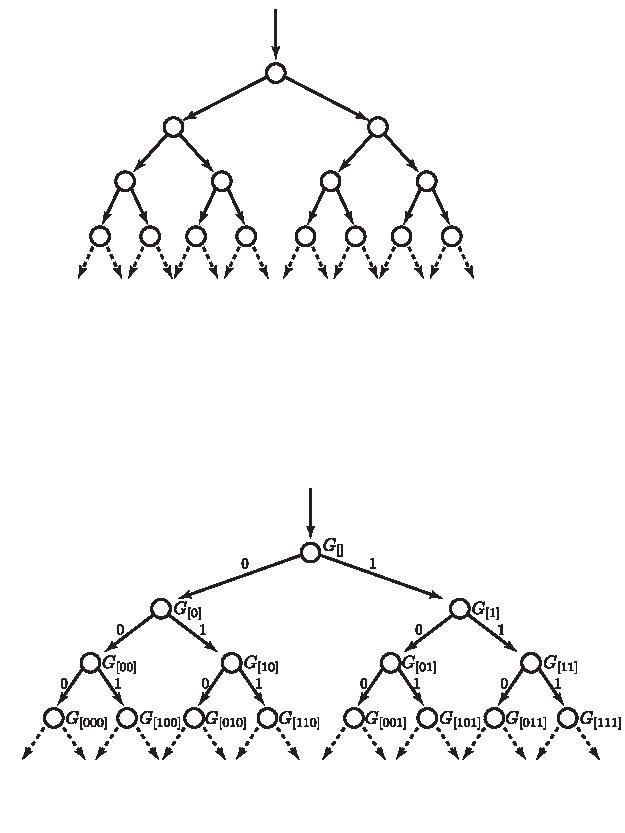
\includegraphics[trim = 4cm 8cm 4cm 8cm, clip, width=5cm]{jtfig/base.pdf}
\vspace{2cm}
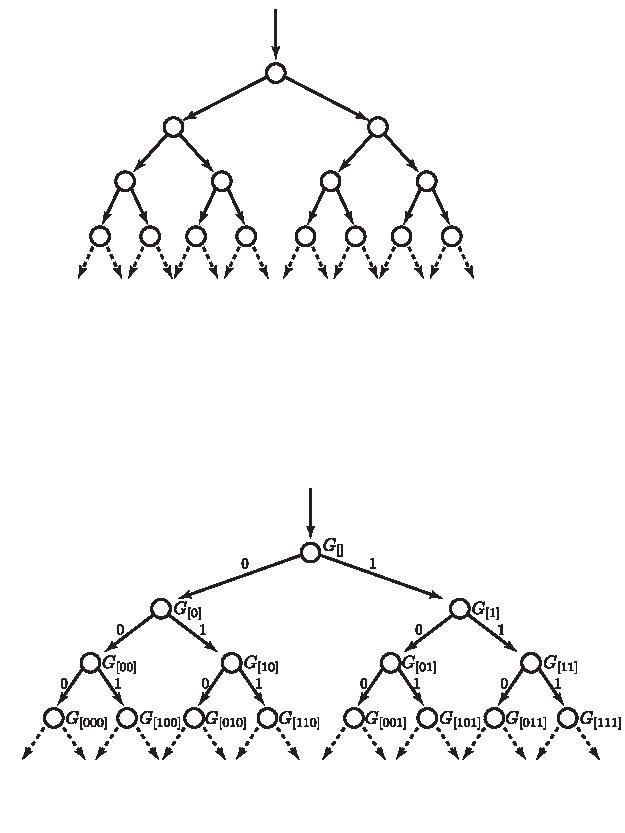
\includegraphics[trim = 2cm 2cm 2cm 10cm, width=8cm]{jtfig/base.pdf}
%\caption{Test perplexity vs.~number of training observations.}
\label{fig: gm_binary_complete}
\end{center}
\end{figure}
}



\frame[t] {
\frametitle{Pitman-Yor process}

%\frametitle{Pitman Yor Process (PYP) : Definition \citep{Pitman1997a}}
 A Pitman-Yor process $\PY(c,d,H)$ is a distribution over distributions with three parameters
\begin{itemize}
\item A discount $ 0 \le d < 1 $ that controls power-law behavior
\begin{itemize}
\item $d=0$ is Dirichlet process (DP)
\end{itemize}
\item A concentration $c > -d$ 
\item A base distribution $H$  
\end{itemize}
\vspace{.25cm}
 {\em a priori} properties :
\begin{itemize}
\item $\EE[G(s)] = H(s)$
\item $\Var[G(s)] = (1-d)H(s)(1-H(s))$
\end{itemize}

}

\frame[t] {
\frametitle{Pitman-Yor process}
\only<1>{Key ``coagulation'' property: \bigskip

If \[G_2| G_1\sim\py(d_1,0,G_1)\] and \[G_3| G_2\sim\py(d_2,0,G_2)\] then $G_2$ can be analytically marginalized out.
\[G_3|G_1\sim\py(d_1d_2,0,G_1)\] 
}

 \citep{Pitman1999, Ho2006}
}

% \frame[t] {%slide 27
% \frametitle{Sequence Memoizer, \citep{Wood2009}}

%\begin{align}
%\prob_\varepsilon &\sim \py(\disc_0,\prob_0)  \label{eqn:hierbayes}\\
%\prob_\context|\prob_\parent &\sim \py(\disc_{|\context|},\prob_\parent) &&
%\text{for all $\context\in\Sigma^{*}_n\backslash\varepsilon$} \nonumber\\
%x_i|\mathbf{x}_{i-n:i-1}=\context,\prob_\context &\sim \prob_\context &&
%\text{for $i=1,\ldots,T$}  \nonumber
%\end{align}
%}



\subsection{Sequence memoizer = hierarchical PY process \citep{Teh2006a} of unbounded depth.}

 





 
   \frame[t] {%slide 27
  \frametitle{$O(n)$ representation for a particular sequence: 110100}
 \begin{figure}[htbp]
\begin{center}
%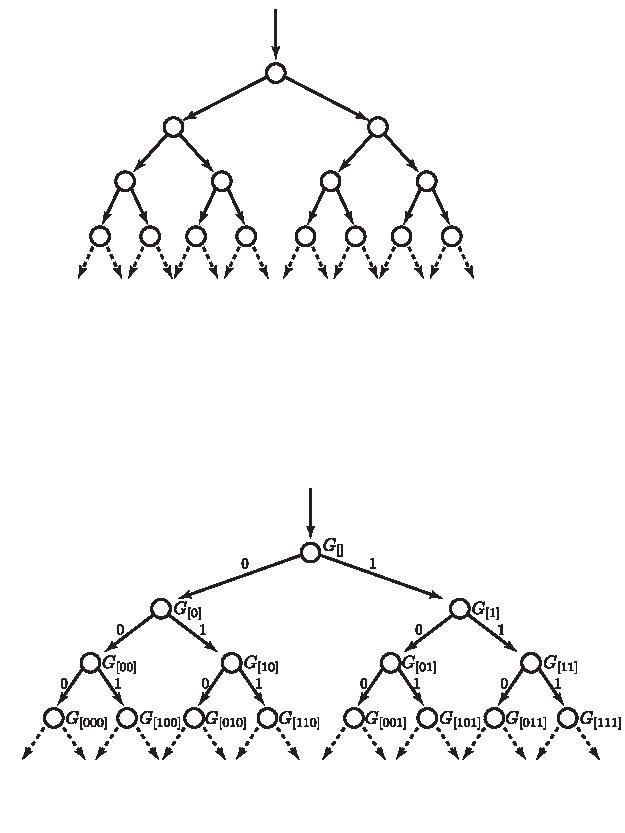
\includegraphics[trim = 4cm 8cm 4cm 8cm, clip, width=5cm]{jtfig/base.pdf}
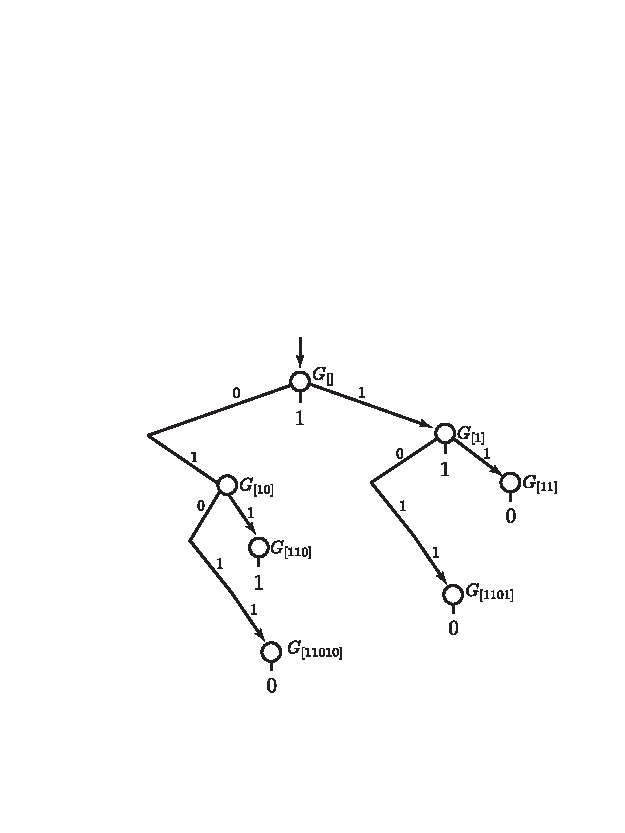
\includegraphics[trim = 2cm 2cm 2cm 6cm, width=8cm]{jtfig/seq_6.pdf}
%\caption{Test perplexity vs.~number of training observations.}
\label{fig: gm_binary_complete}
\end{center}
\end{figure}

 }
 }

%\begin{frame}[t] \frametitle{}
%PY process properties exploited by linear space sequence memoizer.
%\begin{columns}[c] \column{.5\textwidth} 
%\begin{block}{Coagulation \citep{Pitman1999, Ho2006}}
%If \[G_2| G_1\sim\py(d_1,0,G_1)\] and \[G_3| G_2\sim\py(d_2,0,G_2)\] then
%\[G_3|G_1\sim\py(d_1d_2,0,G_1)\] with $G_2$ marginalized out.
%\label{thm:coag}
%\end{block}
%\column{.5\textwidth} 
%\begin{block}{Fragmentation \citep{Pitman1999, Ho2006,Wood2009}}
%Suppose
% \[G_3| G_1\sim\py(d_1d_2,0,G_2)\]
% then $G_3$
% can be ``fragmented'' so 
% \[G_2 | G_1 \sim \py(d_1,0,G_1)\]
% and
%  \[G_3| G_2\sim\py(d_2,0,G_2)\] 
%  if $G_2$ is needed.
%\end{block}
% \end{columns}
% \end{frame}

%\subsection{Inference, crazy-high level overview}
%  \frame[t] {%slide 9
%$\EE[\Gu(s)]$
%is a recursively defined expectation over a set of random counts
%\[\{N(\ubf's'),M(\ubf's')\}_{\ubf'\in\cctx, s'\in\Sigma}\]
%which have properties $M(\ubf's') \leq N(\ubf's')$ and $N(\data_{1:i}x_{i+1}) \geq 1 \; \forall \; i$
%\begin{block}{}
%\vspace{-.5cm}
%\[\EE[\G_\context(s)]
%= \EE\left[
%\frac{N(\context s)-\disc_{\context} M(\context s) + \left(\disc_{\context}\sum_{s'\in\Sigma}  M(\context s')\right) \G_\parent(s)}{\sum_{s'\in\Sigma} N(\context s')}\right]
%\]
% \end{block}
%The counts
%\[\{N(\ubf's'),M(\ubf's')\}_{\ubf'\in\cctx, s'\in\Sigma}\]
%are sampled using sequential Monte Carlo or Markov chain Monte Carlo sampling methods.
%}
%\section{Experiments}
%
%
%\subsection{Compression}
%

\section{Demonstration}


\frame[t]
{
\frametitle{SM versus Smoothed $n^\mathrm{th}$-order Markov model}
\begin{figure}
    \includegraphics[width=.85\columnwidth]{cacm_figs/lm_results}
    \label{fig:sm_vs_ngram}
\end{figure}
\tiny{ SM  versus $n^{\textrm{th}}$ order Markov models with hierarchical PYP priors 
%    $n$-gram model (solid line)
    as $n$ varies.  In red is computational
    complexity.} % (for both the sequence 
%    memoizer (dashed line) and a smoothing $n$-gram model (solid line).
    %For this four million word New York Times corpus, as $n$ passes 4, the memory complexity of the Markov models grows larger than that of the sequence
   % memoizer, yet, the SM model yields modeling
   % performance that is better than all Markov models regardless of their order. %the limit of an $n$-gram as $n\rightarrow\infty$.
  %  This suggests that for $n\ge 4$ the SM model is to be preferred: it
  %  requires less space to store yet results in a comparable if not better
  %  model.
}


\frame[t]
{
\frametitle{Sequence Memoizer application: lossless compression}
\begin{block}{Calgary corpus}
\begin{table}[t]
    \begin{center}
    \setlength{\tabcolsep}{1.3mm}
\begin{tabular}{l||r|c|c|c|c}
%\hline
%\multicolumn{2}{|c||}{} & \multicolumn{2}{c||}{SM} &
%\multicolumn{2}{|c|}{PPM} & CTW\\\hline
\textbf{Model} & SM & PPM & CTW & bzip2 & gzip \\\hline
%File          &  Size  &    1PF    &    UKN    &   PPM* &    PPMZ  &  CTW  \\\hline 
%\hline
%bib           & 111261 &    1.73   &{\bf 1.72}  &   1.91 &    1.74  &  1.83 \\\hline
%book1         & 768771 &{\bf 2.17}  &    2.20   &   2.40 &    2.21  &  2.18 \\\hline
%book2         & 610856 &{\bf 1.83}  &    1.84   &   2.02 &    1.87  &  1.89 \\\hline
%geo           & 102400 &{\bf 4.40}  &    4.40   &   4.83 &    4.64  &  4.53 \\\hline
%news          & 377109 &{\bf 2.20}  &    2.20   &   2.42 &    2.24  &  2.35 \\\hline
%obj1          & 21504  &{\bf 3.64}  &    3.65   &   4.00 &    3.66  &  3.72 \\\hline
%obj2          & 246814 &    2.21   &{\bf 2.19}  &   2.43 &    2.23  &  2.40 \\\hline
%paper1        & 53161  &    2.21   &{\bf 2.20}  &   2.37 &    2.22  &  2.29 \\\hline
%paper2        & 82199  &{\bf 2.18}  &    2.18   &   2.36 &    2.21  &  2.23 \\\hline
%pic           & 513216 &    0.77   &    0.82   &   0.85 &{\bf 0.76} &  0.80 \\\hline
%progc         & 39611  &    2.23   &{\bf 2.21}  &   2.40 &    2.25  &  2.33 \\\hline
%progl         & 71646  &    1.44   &{\bf 1.43}  &   1.67 &    1.46  &  1.65 \\\hline
%progp         & 49379  &    1.44   &{\bf 1.42}  &   1.62 &    1.47  &  1.68 \\\hline
%trans         & 93695  &    1.21   &{\bf 1.20}  &   1.45 &    1.23  &  1.44 \\\hline \hline
%\textbf{avg.} &        &{\bf 2.12}  &    2.12   &   2.34 &    2.16  &  2.24 \\\hline
\textbf{Average bits / byte}      &{\bf 1.89}   & 1.93  &  1.99 & 2.11 & 2.61 \\%\hline
\end{tabular}
\end{center}
\label{table:results}
\end{table}
\end{block}
weighted average log-loss
\[\ell(\xbf_{1:N}) = -\frac{1}{N}\sum_{i=1}^N \log_2 \EE[G(x_i|\xbf_{1:i-1})]\]
(average bits per byte under optimal entropy encoding, lower is better)\footnote{The result for unbounded context-length PPM is from 
\citep{Cleary1997b} and for CTW the result is from \citep{Willems2009}.   The
bzip2 and gzip results come from running the corresponding standard unix
command line tools with no extra arguments.}


}



\frame[t]
{
\frametitle{Compressor based on the sequence memoizer}

\begin{figure}[htbp]
\begin{center}
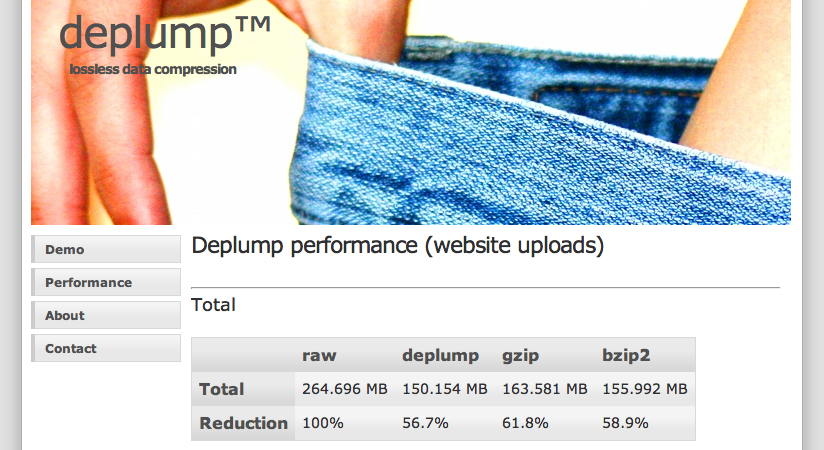
\includegraphics[width=10cm]{deplump_web.png}
\caption{\href{http://www.deplump.com/}{http://www.deplump.com/} }
\label{default}
\end{center}
\end{figure}


%A general purpose streaming lossless compressor (``deplump'') built on the sequence memoizer  is available for demonstration at
%  \begin{itemize}
%  \item \href{http://www.deplump.com/}{http://www.deplump.com/} 
%  \begin{itemize}
%\item    \href{http://www.deplump.com/LookupStatistics}{real time performance} 
%\end{itemize}
%\end{itemize}

}



%\subsection{Language modeling}
%\frame[t]{Language modeling}
%{
%\frametitle{Language modeling}
%
%\begin{block}{}
% \begin{table}
%\begin{center}
%\begin{tabular}[t]{lcc}
%\hline
%{\small Source } & {\small Perplexity\footnote{perplexity = $2^{\mathrm{log\; loss}}$}} \\
%\hline
%{\small Bengio et al.\ \citep{Bengio2003} }& 109.0 \\
%%{\small Mnih \& Hinton \citep{Mnih:NIPS08} } & 112.1 \\
%{\small Mnih et al.\ \citep{Mnih2009}} & \phantom{0}83.9\\
%\hline
%{\small 4-gram Interpolated Kneser-Ney \citep{Chen1999} }& 106.1 \\
%{\small 4-gram Modified Kneser-Ney \citep{Chen1999} }& 102.4 \\
%{\small 4-gram Hierarchical PYP \citep{Teh2006} } & 101.9 \\
%{\small Sequence Memoizer} \citep{Wood2009}& \phantom{0}96.9\\
%\hline
%\end{tabular}
%\end{center}
% %It has
% %been reported that the aspects of the data that are modelled by these two
% %distinct classes of models complement each other, so that even higher perfomance
% %can be achieved by combining both types of models.
% % The sequence memoizer outperforms fixed depth smoothing $n$-gram models but is bettered by a more computationally complex model on this data.  }
%\label{table:ap_perplexities}
%\end{table}
%\end{block}
%Language models of an Associated Press news corpus (lower perplexity is better).  Interpolated and
% modified Kneser-Ney are state-of-the-art language models.  Provided for comparison are 
% the results for the models of Bengio et al.\ and Mnih et al.\ which belong to
% a different class of models that learn word representations from data. 
%}




\frame[t] {
\frametitle{Infinite Structured Explicit Duration Hidden Markov Model}
\textbf{Plug-n-Play hidden Markov model (HMM) upgrade}
\begin{itemize}
\item Problem : *
\item Data : *
\item Latent variables : state sequence and state characteristics 
\begin{itemize}
\item observation distribution and duration distribution parameters
\end{itemize}
%\item Parameters : Priors on all latent variable distributions
\item Algorithm : Block Gibbs with forward-backward slice sampling 
\end{itemize}
\pause
\textbf{Nearest parametric comparable}
\begin{itemize}
\item Explicit duration HMM / Hidden Semi-Markov Model \\
\citep{Mitchell95,Murphy02,Yu:2010}
\end{itemize}
\pause
\textbf{Nearest Bayesian nonparametric comparable}
\begin{itemize}
\item Infinite HMM  \citep{Beal:2002,Teh:2006b}
\item Infinite Explicit Duration HMM  \citep{Johnson:2010}
\end{itemize}
}





\frame[t] {
\frametitle{Hidden Markov Models}
Hidden Markov models (HMMs) \citep{Rabiner:1989} are an important tool for data exploration and engineering applications.
\newline

Applications include
\begin{itemize}
\item Speech recognition \citep{Jelinek97,Juang85}
\item Natural language processing \citep{Manning1999}
\item Hand-writing recognition \citep{Nag1986}
\item DNA and other biological sequence modeling applications \citep{Krogh1994}
\item Gesture recognition \citep{tanguay1995hidden,wilson1999parametric}
\item Financial data modeling \citep{ryden1998stylized}
\item and many more $\ldots$\newline

\end{itemize}

%Assumptions: discrete time, latent Markov process.

}



%\begin{frame}[t]{Example Application: Modeling the Morse Code Cepstrum}
%	\begin{figure}[t]
%		\begin{center}
%			\includegraphics[height = 6cm, transparent]{figs/morse-spectrogram-ED-iHMM-and-iHMM-output}
%		\end{center}
%	\end{figure}
%\end{frame}
%
%\frame[t] {
%\frametitle{Hidden Markov Model Graphical Model}
%\begin{figure}[t]
%		\begin{center}
%			\includegraphics[width = \textwidth, transparent]{figs/HMM-graphical-model}
%		\end{center}
%	\end{figure}
%%An objective: compute the predictive distribution for the next observation:
%%\eqan
%%\lefteqn{P(y_T | y_1,\ldots, y_{T-1}, \{{\bsym\pi}_m\},\{\theta_m\})} \nonumber \\
%%&=& \sum_{z_T}\sum_{z_{T-1}}\cdots\sum_{z_0} p(y_T | z_T) p(z_T | z_{T-1}) \ldots p(y_{1})p(z_{1} | z_{0}) p(z_0) \nonumber
%%\enan
%}


\frame[t] {
\frametitle{Shortcomings of Original HMM Specification}
\begin{itemize}
\item The state cardinality $K$ of the latent Markov chain is usually unknown
\item Latent state dwell times are not usually geometrically distributed
%\eqan
%\lefteqn{P(z_{t} = m, \ldots, z_{t+L} = m )} \nonumber \\
% &=& \prod_{\ell = 1}^L P(z_{t+\ell+1} = m| z_{t+\ell} = m) \nonumber \\
% &=& \mathsf{Geometric}(L; \bsym\pi_m(m)) \nonumber
% \enan
\item Prior knowledge often demands constraints on allowable transitions
\begin{itemize}
\item Chicken pox $\rightarrow$ left-to-right
\end{itemize}

\end{itemize}

}

%\frame[t] {
%\frametitle{Notation: Hidden Markov Model}
%
%\eqan
%%\theta_{m} &\sim& H_{y} \nonumber \\
%\!\!\!\!\! z_{t} | z_{t-1}=m &\sim&
%	\mathsf{Discrete}(\bsym\pi_{m})
%	\nonumber \\
%y_{t} | z_{t}=m &\sim& F_{\theta}(\theta_{m})\nonumber
%\enan
%
%\[\mathbf{A} = \left[ \begin{array}{ccccc}
%	\vdots & & \vdots & & \vdots \\
%	\bsym\pi_{1} &\cdots& \bsym\pi_{m} &\cdots& \bsym\pi_{K} \\
%	\vdots & & \vdots & & \vdots \\
%	\end{array} \right]
%\]
%}
%
%%\frame[t] {
%%\frametitle{Notation: Hidden Markov Model, Choices for $F_{\theta}$}
%%
%%\begin{description}
%%\item[ $F_{\theta} = \mathsf{Multinomial(\Theta)}$] 
%%discrete observations (i.e.~DNA, words, etc.)
%% \[\theta_{m} \; \mbox{is a probability vector}\] 
%% \item[$F_{\theta} = \mathsf{Normal(\Theta)}$] 
%% continuous observations (i.e.~positions, etc.). \[\theta_{m}  = \{\mu_m, \Sigma_m\}\]
%%\end{description}
%%
%%
%%
%%%We define the observation sequence $\mathcal{Y} = \{y_1, y_2, \ldots, y_T\}$; the latent state sequence $\mathcal{X} = \{x_0, x_1, x_2, \ldots, x_T\}$; and the remaining time in each segment $\mathcal{D} = \{ d_1, d_2, \ldots, d_T\}$, where $x_t \in \{ 1, 2, \ldots, K\}$ with $K$ the maximum number of states, $d_t \in \{1, 2, \ldots \}$, and $y_t \in \mathbb{R}^n$.     We assume that the Markov chain on the latent states is homogenous, i.e., that $p(x_t = i | x_{t-1}=j, A) = a_{i,j} \forall t$ where $A$ is a $K\times K$ matrix with element $a_{i,j}$ at row $i$ and column $j.$  
%%
%%}
%
%%\frame[t] {
%%\frametitle{ HMM: Dynamic mixture model}
%% \begin{figure}[t]
%%		\begin{center}
%%			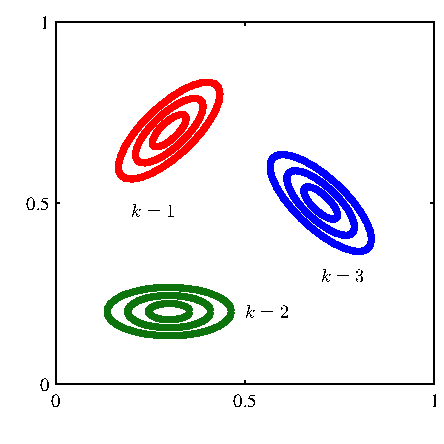
\includegraphics[width = .5\textwidth, transparent]{figs/Figure13_8a}
%%			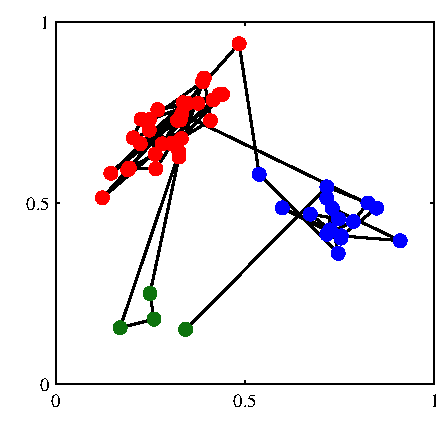
\includegraphics[width = .5\textwidth, transparent]{figs/Figure13_8b}
%%		\end{center}
%%	\end{figure}
%%	Visualization from PRML. \citep{Bishop06}
%%
%%}
%
%%\frame[t] {
%%\frametitle{ HMM: Trellis}
%% \begin{figure}[t]
%%		\begin{center}
%%			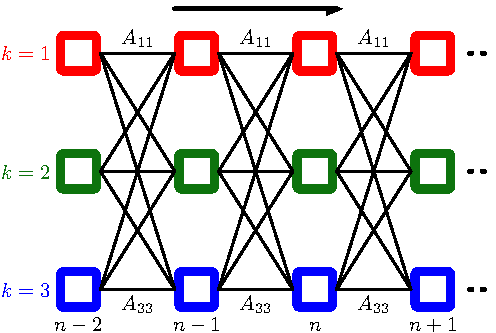
\includegraphics[width = .7\textwidth, transparent]{figs/Figure13_7}
%%		\end{center}
%%	\end{figure}
%%	Visualization from PRML. \citep{Bishop06}
%%
%%}
%
%
%\frame[t] {
%\frametitle{HMM: Typical Usage Scenario (Character Recognition)}
%\begin{itemize}
%\item Training data: multiple ``observed''  $y_t = \{v_t,h_t\}$ sequences of stylus positions for each kind of character %(stroke boundaries unobserved but important ``structurally'' --- correspond to latent states)
%\item Task: train $|\Sigma|$ different models, one for each character %(Maximum likelihood training via EM: {\em Baum-Welch} \citep{baum1972equality}, {\em forward-backward} \citep{Rabiner:1989}, belief propagation \citep{Bishop06})
%\item Latent states: sequences of strokes 
%\item Usage: classify new stylus position sequences using trained models  $\mathcal{M}_\sigma = \{A_\sigma, \Theta_\sigma\}$% and Bayes factors
%\[ P(  \mathcal{M}_\sigma | y_1,\ldots,y_T) \propto P(y_1,\ldots,y_T | \mathcal{M}_\sigma) P( \mathcal{M}_\sigma) \]
% %which requires marginalizing out $z$'s 
%%\[ P(y_1,\ldots,y_T | \mathcal{M}_\sigma) = \sum_Z P(y_1,\ldots,y_T, z_0, \ldots, z_T | A_\sigma, \Theta_\sigma)\]
%\end{itemize}
%
%}
%

%
%%\section{Related Work}
%
%%\frame[t] {
%%\frametitle{Explicit Duration HMM / H. Semi-Markov Model}
%%\citep{Mitchell95,Murphy02,Yu03,Yu:2010}
%%\begin{itemize}
%%\item Latent state sequence $\bsym z = (\{s_{1},r_1\},\dots, \{s_{T},r_T\})$
%%\item Latent state id sequence $\bsym s = (s_{1},\dots, s_{T})$
%%\item Latent ``remaining duration'' sequence $\bsym r = (r_{1},\dots, r_{T})$
%%%\item Observation sequence $\bsym y = (y_{1}, \dots, y_{T})$
%%\item State-specific duration distribution $F_{r}(\lambda_{m})$
%%%\item State transition matrix with columns $\bsym \pi_{m} = (\pi_{m1},\pi_{m2},\dots, \pi_{mM})$
%%%\item State-specific observation distribution $y_{t} \sim F_{\theta}(\theta_{m})$
%%\item Other distributions the same
%%\end{itemize}
%%
%%An EDHMM transitions between states in a different way than does a typical HMM. Unless $r_{t} = 0$  the current remaining duration is decremented and the state does not change.  If $r_{t} = 0$ then the EDHMM transitions to a state $m \ne s_{t}$ according to the distribution defined by $\bsym \pi_{s_{t}}$ 
%%
%%%A finite explicit duration HMM (EDHMM) consists of a hidden state sequence $\bsym s = (s_{1},\dots, s_{T})$, the corresponding observation sequence $\bsym y = (y_{1}, \dots, y_{T})$, and a latent ``remaining duration'' sequence $\bsym r = (r_{1},\dots, r_{T})$.  It also has a state transition matrix  $\bsym \pi$, where the row vector $\bsym \pi_{m} = (\pi_{m1},\pi_{m2},\dots, \pi_{mM})$ corresponds to the transition probabilities out of state $m$, and $\bsym \pi_{0}$ is the initial state vector. An EDHMM transitions between states in a different way than does a typical HMM. Unless $r_{t} = 0$  the current remaining duration is decremented and the state does not change.  If $r_{t} = 0$ then the EDHMM transitions to a state $m \ne s_{t}$ according to the distribution defined by $\bsym \pi_{s_{t}}$. The duration the HMM will remain in the new state $m$ is drawn from the  state-specific duration distribution $F_{r}(\lambda_{m})$ governed by parameter $\lambda_{m}$. At each timestep the observation $y_{t} \sim F_{\theta}(\theta_{m})$ is drawn from a state-specific emission distribution parameterized by $\theta_{m}$.   The emission distribution parameters are given a shared prior $\theta_m \sim H_{\theta}$. The IEDHMM is an EDHMM with a countable number of states, i.e.~$M\rightarrow\infty$.
%%
%%
%%}
%
%\frame[t] {
%\frametitle{EDHMM notation}
%
%Latent state $z_t = \{s_t, r_t\}$ is tuple consisting of state identity and time left in state.
%
%\eqan
%%\theta_{m} &\sim& H_{\theta} \nonumber \\
%%\lambda_{m} &\sim& H_{r}\nonumber \\
%\!\!\!\!\! s_{t} | s_{t-1}, r_{t-1} &\sim& 
%	\begin{cases} 
%	\mathbb I(s_{t} = s_{t-1}), & \! r_{t-1} > 0 \\
%	\mathsf{Discrete}(\bsym\pi_{s_{t-1}}), & r_{t-1} = 0
%	\end{cases}\nonumber \\
%\!\!\!\!\! r_{t } | s_{t}, r_{t-1} &\sim& 
%	\begin{cases} 
%	\mathbb I(r_{t} = r_{t-1} - 1),& r_{t-1} > 0 \\
%	F_{r}(\lambda_{s_{t}}),& r_{t-1} = 0
%	\end{cases} \nonumber\\
%y_{t} | s_{t} &\sim& F_{\theta}(\theta_{s_{t}})\nonumber
%\enan
%
%
%}
%
%\frame[t] {
%\frametitle{EDHMM: Graphical Model}
%\begin{figure}[t]
%		\begin{center}
%			\includegraphics[width = \textwidth, transparent]{figs/EDHMM-graphical-model}
%		\end{center}
%	\end{figure}
%}
%
%
%
%
%
%\frame[t] {
%\frametitle{Structured HMMs: i.e.~left-to-right HMM \citep{Rabiner:1989}}
%
%\begin{block}{Example: Chicken pox}
%\begin{description}
%\item[Observations] vital signs
%\item[Latent states] pre-infection, infected, post-infection\footnote{disregarding shingles} 
%\item[State transition structure]  can't go from infected to pre-infection
%\end{description}
%\end{block}
%Structured transitions imply zeros in the transition matrix $A$, i.e.
%
%\[p(s_t = m | s_{t-1} = \ell) = 0 \; \forall \; m < \ell\]
%
%
%}
%
%
%%\frame[t] {
%%\frametitle{Structured HMM: Trellis: One step at a time, left-to-right HMM }
%%
%% \begin{figure}[t]
%%		\begin{center}
%%			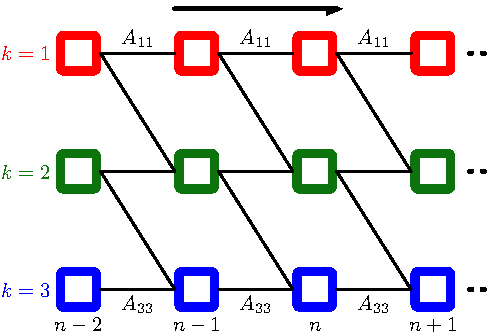
\includegraphics[width = .7\textwidth, transparent]{figs/Figure13_10}
%%		\end{center}
%%	\end{figure}
%%	Figure from PRML. \citep{Bishop06}
%%
%%}
%
%\frame[t] {
%\frametitle{Bayesian HMM}
%
%\begin{itemize}
%\item We will put a {\em prior} on parameters so that we can effect a solution that conforms to our  ideas about what the solution should look like 
%
%\begin{itemize}
%\item Structured prior examples
%\begin{itemize}
%\item $A_{i,j}=0$ (hard constraints)
%\item $A_{i,j}\approx \sum_j A_{i,j}$ (rich get richer)
%\end{itemize}
%\end{itemize}
%
%
%\item  {\em Regularization} means that we can specify a model with more parameters than could possibly be needed
%\begin{itemize}
%\item infinite complexity  (i.e.~$K \rightarrow \infty$) avoids many model selection problems
%\item  ``extra'' states can be thought of as auxiliary or nuisance variables 
%\end{itemize}
%%\item  Posterior inference treats parameters $A$ and $\Theta$ as latent variables
%
%\end{itemize}
%
%
%}
%
%%\frame[t] {
%%\frametitle{Bayesian HMM}
%% Posterior inference treats parameters as latent variables and marginalizes them out too. \newline
%%
%%%Consider the earlier sequence classification task, now
%%
%%%\[P(\{y_1,\ldots,y_T\}^{\mbox{new}} |  \]
%%%
%%%\[ P(  \mathcal{M}_\sigma | y_1,\ldots,y_T) \propto P(y_1,\ldots,y_T | \mathcal{M}_\sigma) P( \mathcal{M}_\sigma) \]
%%% which requires marginalizing out $z$'s {\em and} $A$ and $\Theta$
%%%\eqan
%%%\lefteqn{P(y_1,\ldots,y_T | \mathcal{H})}\nonumber \\
%%%&=& \int \int \sum_Z P(y_1,\ldots,y_T, z_0, \ldots, z_T,  A_\sigma, \Theta_\sigma| \mathcal{H}) dP(A_\sigma) dP(\Theta_\sigma)
%%%\enan
%%%where $\mathcal{H}$ is a set of hyperparameters.
%%
%%
%%
%%}
%
%\frame[t] {
%\frametitle{Bayesian HMM}
%\begin{figure}[t]
%		\begin{center}
%			\includegraphics[width = \textwidth, transparent]{figs/Bayesian-HMM-graphical-model}
%		\end{center}
%	\end{figure}
%%
%\alert<1>{\eqan
%\bsym\pi_{m} &\sim& H_{z} \nonumber \\
%\theta_{m} &\sim& H_{y} \nonumber 
%\enan}%
%\eqan
%\!\!\!\!\! z_{t} | z_{t-1}=m &\sim&
%	\mathsf{Discrete}(\bsym\pi_{m})
%	\nonumber \\
%y_{t} | z_{t}=m &\sim& F_{\theta}(\theta_{m})\nonumber
%\enan
%}
%
%
%\frame[t] {
%\frametitle{Infinite HMMs (IHMM) \citep{Beal:2002,Teh:2006b}}
% 
% 
% 
% \begin{figure}[t]
%		\begin{center}
%			\includegraphics[width = \textwidth, transparent]{figs/iHMM-graphical-model}
%		\end{center}
%	\end{figure}
%	  \[K \rightarrow \infty\]
%
%}
%
%\frame[t] {
%\frametitle{Other HMM variants}
%\begin{itemize}
%\item Sticky Infinite HMMs \citep{Fox:2010tg}
%\begin{itemize}
%\item Extra parameter per state used to bias towards self-transition
%\end{itemize}
%\item Hierarchical HMMs \citep{Murphy01a} 
%\begin{itemize}
%\item State is hierarchical (i.e.~sequence of letters composed of stroke sequences)
%\end{itemize}
%\item  Factorial HMMs \citep{Ghahramani96a}
%%\begin{itemize}
%%\item State is binary encoding 
%%\end{itemize}
%\item  Infinite explicit duration HMM \citep{Johnson:2010}
%\begin{itemize}
%\item No generative model. Latent history sampling used to assert the existence of an implicitly defined IEDHMM that can be sampled from by rejecting HDP-HMM samples that violate transition constraints.
%\end{itemize}
%\end{itemize}
%
%}
%
%\section{ISEDHMMs}
%
%
%
%
\frame[t] {
\frametitle{Infinite Structured Explicit Duration HMM (ISEDHMM) }

Generalized HMM with
\begin{itemize}
\item Infinite state cardinality
\item Explicitly parameterized duration distributions
\item Structured transitions
\end{itemize}
%Fundamental Problems
%\begin{itemize}
%\item How to generate {\em structured, dependent, infinite-dimensional} transition distributions.
%\begin{itemize}
%\item Example: explicit duration HMM's require no self-transitions \[\bsym\pi_i(i)=A_{i,i}=0\]
%\item HDP-HMM construction good for dependence, doesn't work for structure
%\end{itemize}
%The HDP-HMM construction of the iHMM  \citep{Teh:2006b, VanGael:2008} would seem to be a good way to construct an IEDHMM. 
%In sich a construction each row of $\bsym\pi$ (of which there a countably infinite number) would be a draw from a Dirichlet process (DP) with base measure $D_{0} = \sum_{k=1}^{\infty} w_{k}\delta_{\theta_{k}}$, where $D_{0}$ is itself a draw from a Dirichlet process with base measure $H_{\theta}$.
%Therefore, the $m$-th draw $D_{m} \sim \textnormal{DP}(c_{0}D_{0})$ can be written as $D_{m} = \sum_{k} \pi_{mk}\delta_{\theta_{k}}$. 
%Unfortunately the IEDHMM cannot be constructed in this manner because the HPD-HMM cannot enforce the kind of dependence required by the no self-transition condition $m \ne s_{t}$.  This is because the HDP prior on the transition distributions requires that any time a state is transitioned to from any other state it becomes more likely to be transitioned to by all other states.  Unfortunately developing a a model in which the state transition distributions exhibit dependence on a covariate or auxiliary variable requires the abandoning the conditional independence requirement of the HDP.
%\item How to do inference in HMMs with countable state cardinality and countable duration distribution support.
%\end{itemize}
\;\;\;\;\;\;\citepalias{Huggins-2012-AISTATS}
}



%\begin{frame}[t]{ ISEDHMM: Graphical Model}
%	\begin{figure}[t]
%		\begin{center}
%			\includegraphics[height = 5cm, transparent]{figs/ED-iHMM-graphical-model}
%		\end{center}
%	\end{figure}
%	
%	{\em Structured, dependent, infinite-dimensional} transition distributions?
%\end{frame}

\frame[t] {
\frametitle{ISEDHMM: Recipe}
\begin{itemize}
\item Poisson process \citep{Kingman:1993} 
\item Gamma process \citep{Kingman:1993} 
\item SN\GP s \citep{Rao:2009}
\center{$\Downarrow$}
\item {\em Structured, dependent, infinite-dimensional} transition distributions \citepalias{Huggins-2012-AISTATS}
\end{itemize}

}

%\frame[t] {
%\frametitle{ISEDHMM: Recipe}
%
%\begin{itemize}
%\item Gamma process  \citep{Kingman:1993} as Poisson process over $\Theta \otimes V \otimes [0,\infty)$ with rate / mean measure
%\eqn \mu(\tilde\Theta, \tilde V,  \tilde S) = \alpha(\tilde\Theta, \tilde V) \int_{\tilde S}\gamma^{-1}e^{-\gamma} \nonumber \enn
%\item A draw from a Gamma process with \[\alpha(\tilde\Theta,  \tilde V) = c_{0}H_{\theta}(\tilde\Theta)H_{v}( \tilde V).\] \citep{Kingman:1993} has the form
%\eqn G  = \sum_{m=1}^{\infty} \gamma_{m} \delta_{(\theta_{m}, v_{m})} \nonumber \enn
%where $(\theta_{m}, v_{m}) \sim H_{\theta}\times H_{v}$. \newline
%\end{itemize}
%
%}
%\frame[t] {
%\frametitle{ISEDHMM: Recipe}
%\begin{itemize}
%\item Non-disjoint ``restricted projections'' of Gamma processes are {\em dependent} Gamma processes (SN\GP s) \citep{Rao:2009}
%\begin{figure}[t]
%		\begin{center}
%			\includegraphics[width=.75\textwidth, transparent]{figs/isedhmm_geom_base_gp}
%		\end{center}
%	\end{figure}
%	
%	\end{itemize}
%
%\eqn G_0 = \sum_{m\neq0} \ldots, \;\;\;\cdots\;\;\;,G_4  = \sum_{m\neq4} \gamma_{m} \delta_{\theta_{m}},\;\;\;\cdots\;\;\;  \nonumber \enn
%
%}
%	
%	
%\frame[t] {
%\frametitle{ISEDHMM: Recipe}
%
%	\begin{itemize}
%
%\item Normalized dependent \GP~draws are dependent Dirichlet process draws.\footnote{a draw from a Dirichlet process \citep{Ferguson1973} is an infinite sum of weighted atoms \citep{Sethuraman1994} where the weights sum to one.}  In the ISEDHMM, DP draws are the dependent, structured, infinite-dimensional transition distributions
%
%\eqan D_4  &=& \frac{G_4}{G_4(\Theta)} \\
% &=& \frac{\sum_{m\neq4} \gamma_{m} \delta_{\theta_{m}}}{\sum_{\theta \in \Theta}\sum_{m'\neq4} \gamma_{m'} \delta_{\theta_{m'}}} \\
% &=& \frac{\sum_{m\neq4} \gamma_{m} \delta_{\theta_{m}}}{\sum_{m'\neq4} \gamma_{m'}}\\
% &=& \sum_{m\neq4} \frac{\gamma_{m}}{\sum_{m'\neq4} \gamma_{m'}} \delta_{\theta_{m}} \nonumber \enan
%	\end{itemize}
%
%}
%
%\frame[t] {
%\frametitle{ISEDHMM: Recipe}
%	\begin{figure}[t]
%		\begin{center}
%			\includegraphics[height = 6cm, transparent]{figs/ED-iHMM-hierarchical-model}
%		\end{center}
%	\end{figure}
%	
%	\begin{itemize}
%
%\item Structured, dependent, infinite dimensional transition distributions $\bsym\pi_m$ can be formed from draws from DDPs \citepalias{Huggins-2012-AISTATS}
%%\item Auxiliary variables
%%\item Beam Sampling
%\end{itemize}
%}

%\begin{frame}[t]{IEDHMM: Geometric base distribution over states example}
%	\end{frame}

%\frame[t] {
%\frametitle{Structured Transitions Via Dependent Dirichlet Processes}
%\begin{itemize}
%\item<1-3> One way to define a set of dependent DPs is to construct a base gamma process over an augmented space by taking the union of disjoint independent gamma processes, then define a series of restricted projections of that base process, which are themselves gamma processes. 
%
%\item<2-3> The normalization of these dependent gamma processes form a set of dependent DPs.  
%
%\item<3-3> We will use this procedure to construct a number of dependent DPs (one for each HMM state) which preclude certain transitions.  The precluded transitions, a form of dependence,  arise from particulars.
%\end{itemize}
%
%}


\frame[t] {
\frametitle{ISEDHMM Inference: Beam Sampling}
Forward-filtering, backward slice-sampling approach for the IHMM of \citep{VanGael:2008} and EDHMM of \citepalias{Dewar:2011} %This so-called beam sampling approach is an auxiliary variable slice-sampling approach. 
\bigskip

Gist :
\newline

State and duration variables are sampled conditioned on auxiliary slice variables \bigskip % via a forward-chainin 

Take home : 
\newline

Efficient, always finite forward backward procedure for sampling latent states

}

%
%
%\frame[t] {
%\frametitle{Auxiliary Variables for Sampling}
%\begin{columns}[t]
%\begin{column}{.5\textwidth}
%
%Objective: get samples of $x$.  \newline 
%
%\uncover<2->{Sometimes it is easier to introduce an auxiliary variable $u$ and to Gibbs sample the joint $P(x,u)$ (i.e.~sample from $P(x|u; \lambda)$ then $P(u|x, \lambda)$, etc.) then discard the $u$ values than it is to directly sample from $p(x|\lambda)$. \newline}%
%
%\uncover<3->{Useful when: $p(x|\lambda)$ does not have a known parametric form but adding $u$ results in a parametric form {\em and} when $x$ has countable support and sampling it requires enumerating all values. }
%
%	\end{column}
%	\begin{column}{.25\textwidth}
%\uncover<1->{\begin{figure}[t]
%		\begin{center}
%			\includegraphics[height = 3cm, transparent]{figs/poisson_slice_sampling_example_before_aux}
%		\end{center}
%	\end{figure}
%	}
%	\end{column}
%		\begin{column}{.25\textwidth}
%
%	\uncover<2->{\begin{figure}[t]
%		\begin{center}
%			\includegraphics[height = 5cm, transparent]{figs/poisson_slice_sampling_example}
%		\end{center}
%	\end{figure}
%	}
%	\end{column}
%	\end{columns}
%
%
%}
%
%
%
%
%\frame[t] {
%\frametitle{Slice Sampling: A {\em very} useful auxiliary variable sampling trick}
%Unreasonable Pedagogical Example: 
%\begin{itemize}
%\item $x|\lambda \sim \mathsf{Poisson}(\lambda)$ (countable support)
%\item  {\em enumeration} strategy for sampling $x$ (impossible)
%\item auxiliary variable $u$ with $P(u|x,\lambda) = \frac{\mathbb{I}(0 \leq u \leq P(x|\lambda))}{P(x|\lambda)}$
%\end{itemize}
%Note:
%Marginal distribution of $x$ is 
%\eqan
%P(x|\lambda) &=& \sum_u P(x,u|\lambda) \nonumber\\
%&=& \sum_u P(x|\lambda)P(u|x,\lambda) \nonumber\\
%&=& \sum_u P(x|\lambda) \frac{\mathbb{I}(0 \leq u \leq P(x|\lambda))}{P(x|\lambda)}\nonumber\\
%&=& \sum_u \mathbb{I}(0 \leq u \leq P(x|\lambda)) = P(x|\lambda) \nonumber
%\enan
%
%}
%
%\frame[t] {
%\frametitle{Slice Sampling: A {\em very} useful auxiliary variable sampling trick}
%This suggests a Gibbs sampling scheme: alternately sampling from
%\begin{itemize}
%\item $P(x|u,\lambda) \propto \mathbb{I}(u \leq P(x|\lambda))$ 
%\begin{itemize}
%\item {\em finite} support, uniform above slice, enumeration {\em possible}
%\end{itemize}
%\item  $P(u|x,\lambda) = \frac{\mathbb{I}(0 \leq u \leq P(x|\lambda))}{P(x|\lambda)}$ 
%\begin{itemize}
%\item uniform between 0 and $y=P(x|\lambda)$
%\end{itemize}
%\end{itemize}
%then discarding the $u$ values to arrive at $x$ samples marginally distributed according to $P(x|\lambda)$.
%}
%
%\frame[t] {
%\frametitle{ISEDHMM Inference: Beam Sampling}
%Forward-backward slice sampling only has to consider a finite number of successor states at each timestep.  With auxiliary variables
%
%\eqn p(u_{t} | z_{t}, z_{t-1}) = \frac{\mathbb I(u_{t} < p(z_{t} | z_{t-1}))}{ p(z_{t} | z_{t-1})} \nonumber \enn
%
%and
%
%\eqan
% p(z_{t} | z_{t-1}) &=&
% p((s_t , r_t ) | (s_{t-1}, r_{t-1}))  \nonumber \\
%	&=&\begin{cases} 
%	r_{t-1} > 0, & \mathbb{I}(s_t=s_{t-1})\mathbb{I}(r_t = r_{t-1}-1) \\
%	r_{t-1} = 0, & \pi_{s_{t-1}s_{t}}F_r(r_t;\lambda_{s_t}).
%	\end{cases} \nonumber 
%\enan
%
%one can run standard forward-backward conditioned on $u$'s.
%}

\frame[t] {
\frametitle{ISEDHMM Inference : Synthetic Data Example}
Data from a 4 state EDHMM with Poisson duration distribution means \[\bsym \lambda = (10, 20, 3, 7)\] and unit-variance Gaussian emission distributions with means \[\bsym \mu = (-6, -2, 2, 6)\] 
}

\begin{frame}[t]{IEDHMM Inference : Synthetic Data Results}
	\begin{figure}[t]
		\begin{center}
			\includegraphics[height = 7cm, transparent]{figs/combined-overlay-state-distribution-figure}
		\end{center}
	\end{figure}
\end{frame}

\begin{frame}[t]{IEDHMM: Synthetic Data, State Duration Parameter Posterior }
	\begin{figure}[t]
		\begin{center}
			\includegraphics[height = 6cm, transparent]{figs/4-states-4-apart-1-variance-duration-posteriors-big-font}
		\end{center}
	\end{figure}
\end{frame}

\begin{frame}[t]{IEDHMM: Synthetic Data, State Mean Posterior}
	\begin{figure}[t]
		\begin{center}
			\includegraphics[height = 6cm, transparent]{figs/4-states-4-apart-1-variance-mean-posteriors-big-font}
		\end{center}
	\end{figure}
\end{frame}

\begin{frame}[t]{IEDHMM: Nanoscale Transistor Spontaneous Voltage Fluctuation}
	\begin{figure}[t]
		\begin{center}
			\includegraphics[height = 6cm, transparent]{figs/RTS-ED-iHMM-overlay}
		\end{center}
	\end{figure}
\end{frame}



\begin{frame}[t]{IEDHMM vs. IHMM:  Modeling the Morse Code Cepstrum}
	\begin{figure}[t]
		\begin{center}
			\includegraphics[height = 6cm, transparent]{figs/morse-spectrogram-ED-iHMM-and-iHMM-output}
		\end{center}
	\end{figure}
\end{frame}



\begin{frame}[t]{Wrap-Up}
\begin{itemize}
\item Applied statistical machine learning research is about abstracting problems such that they can be solved using abstract models and inference algorithms.
\item Statistical machine learning research is about developing re-usable, expressive models and computationally tractable inference algorithms.
\item The sequence memoizer and ISEDHMM are two new reusable, highly expressive, computationally-tractable Bayesian nonparametric models.
\end{itemize}

\end{frame}



\begin{frame}[t]{Future Work}
Agents attempting to accrue reward through action need highly expressive, computationally efficient probabilistic models to represent and do inference about the state of the world.
\begin{figure}[htbp]
\begin{center}

\includegraphics[width = .25\textwidth, transparent]{stock/39298bupheonw6vt.png}
\hspace{2cm}
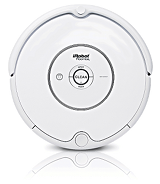
\includegraphics[width = .125\textwidth, transparent]{stock/iRobot_Roomba_530_270x310t.png}
\label{fig:actors}
\end{center}
\end{figure}
\vspace{.25cm}
\center{\tiny{Credit: (left) digitalart / FreeDigitalPhotos.net (right) iRobot Corporation}}

%\begin{itemize}
%\item Generalize to spatial prior on HMM states (``location'')
%\begin{itemize}
%\item Simultaneous location and mapping
%\item Process diagram modeling for systems biology
%\end{itemize}
%\end{itemize}
\end{frame}

%\frame[t] {
%\frametitle{AI: Accrue reward by acting in the world. }
%
%\begin{figure}[htbp]
%\begin{center}
%
\includegraphics[width = .25\textwidth, transparent]{stock/39298bupheonw6vt.png}
%\hspace{2cm}
%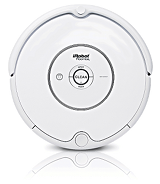
\includegraphics[width = .125\textwidth, transparent]{stock/iRobot_Roomba_530_270x310t.png}
%\label{fig:actors}
%\end{center}
%\end{figure}
%\vspace{2cm}
%\center{\tiny{Credit: (left) digitalart / FreeDigitalPhotos.net (right) iRobot Corporation}}
%}


%\frame[t] {
%\frametitle{Partially Observable Markov Decision Process}
%Unsupervised learning in control
%\begin{figure}[htbp]
%\begin{center}
%Action, perception cycle graphic.
%\label{fig:actors}
%\end{center}
%\end{figure}
%\vspace{2cm}
%\center{\tiny{Images: Master isolated images, David Castillo Dominici,  / FreeDigitalPhotos.net}}
%}

\frame[t] {
\frametitle{POMDP : Motivation to Develop Ever More Expressive Models}

\begin{figure}[htbp]
\begin{center}
\includegraphics[width=9cm]{action_reward_cycle.pdf}
\label{fig:actors}
\end{center}
\end{figure}
\vspace{2cm}
\center{\tiny{Images: Master isolated images, David Castillo Dominici,  / FreeDigitalPhotos.net}}
}

%\frame[t] {
%\frametitle{Opinion: best justification for Bayesian nonparametrics}
%\begin{itemize}
%\item Highly expressive models whose expressivity grows with data size.
%\item Framework for performing inference directly about complex entities.
%\end{itemize}
%
%}



%\frame[t] {
%\frametitle{HMM as PNFA}
%}
%
%\frame[t] {
%\frametitle{Computational Models of Worlds}
%}
%
%\frame[t] {
%\frametitle{Sequence Memoizer}
%}
%
%\frame[t] {
%\frametitle{Probabilistic Deterministic Infinite Automata}
%}
%
%
%
%\begin{frame}[t]{Sequence Memoizer graphical model ``oacac" \citep{Wood2009}}
%	\begin{figure}[t]
%		\begin{center}
%			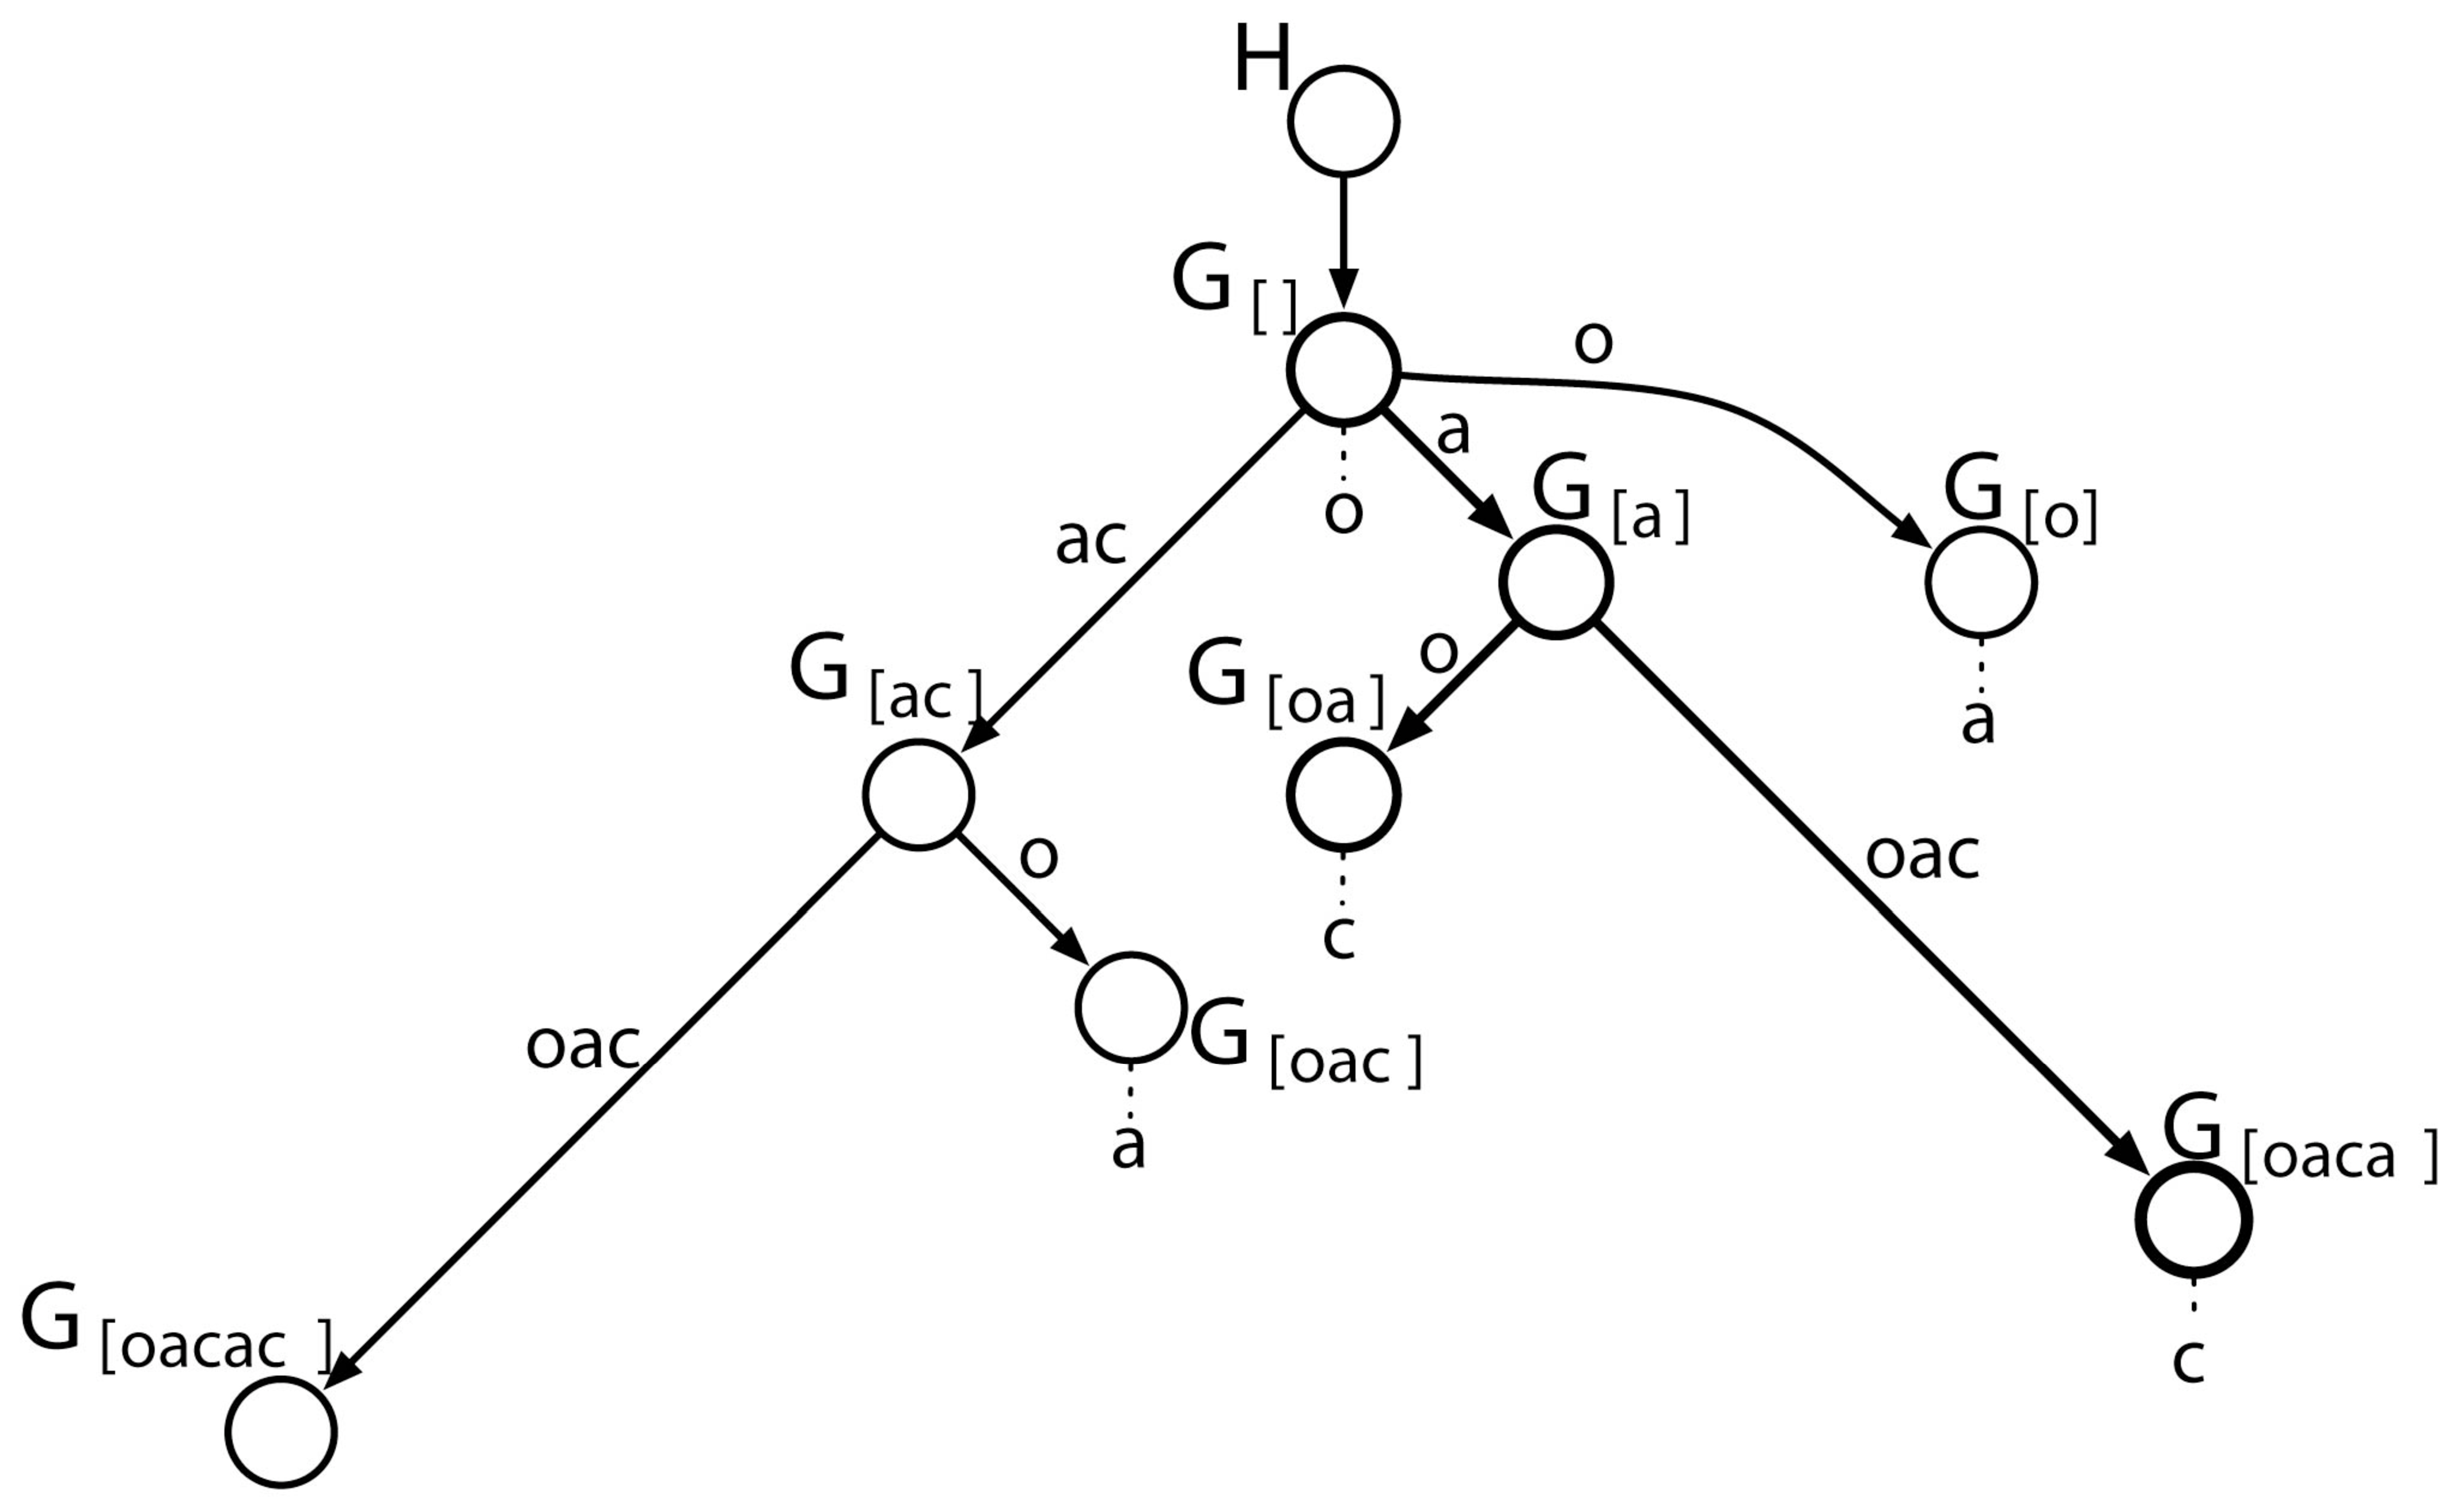
\includegraphics[height = 6cm, transparent]{figs/prefix_tree_not_coloured.pdf}
%		\end{center}
%	\end{figure}
%\end{frame}
%
%\begin{frame}[t]{Full Corpus Compression}
%
%	   	\begin{figure}[t]
%		\begin{center}
%			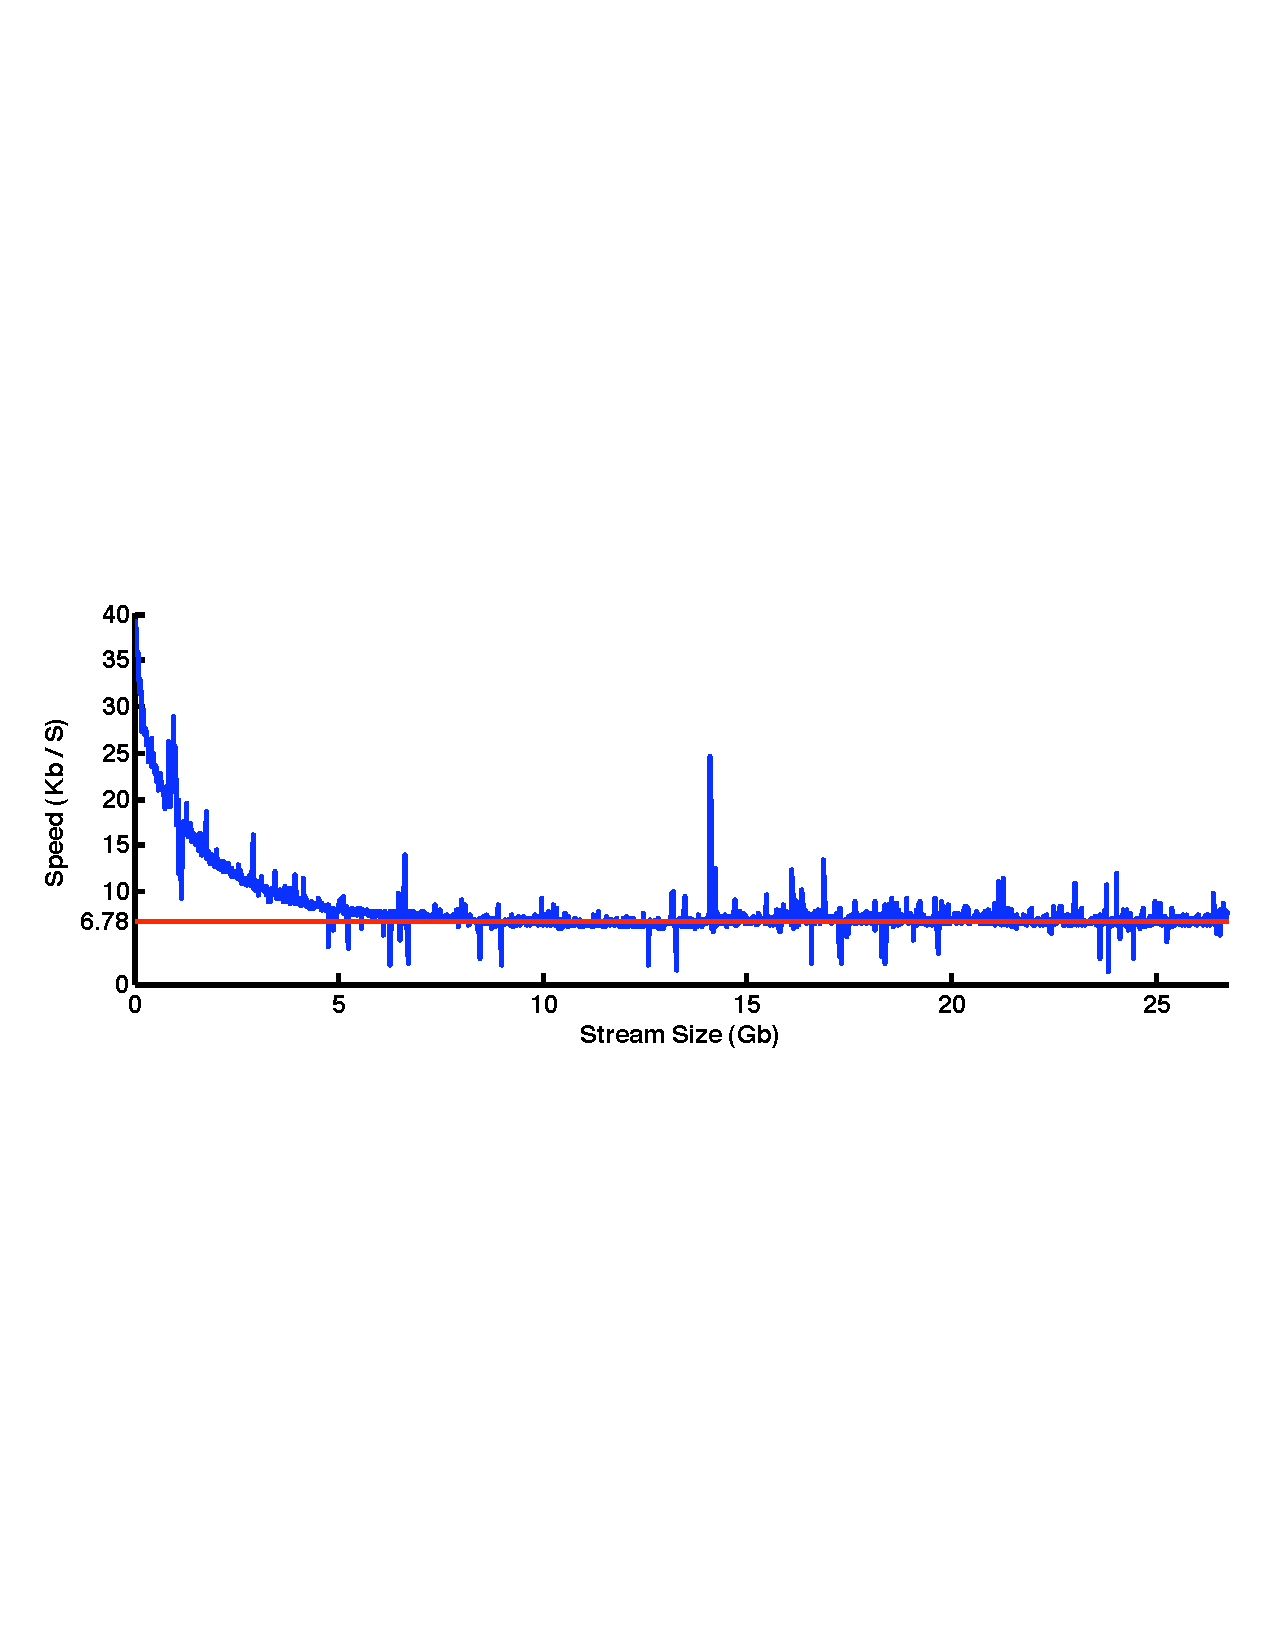
\includegraphics[width = 11cm]{figs/constant_speed_asymptote_small.pdf}
%		\end{center}
%	\end{figure}
%
%First streaming SM with computational asymptotics required for streaming compression.  Compressed 26.8Gb Wikipedia corpus to 4Gb (vs. 7.9Gb for gzip and 3.8Gb for PAQ).
%
%\end{frame}
%
%
%\begin{frame}[t]{ IEDHMM vs. IHMM }
%	\begin{figure}[t]
%		\begin{center}
%			\includegraphics[width = .45\textwidth, transparent]{figs/iHMM-comparison-3d}
%			\includegraphics[width = .45\textwidth, transparent]{figs/iHMM-reverse-comparison-3d}
%		\end{center}
%	\end{figure}
%	{ \tiny Left: data from Poisson duration distribution ISEDHMM, Right: data from IHMM fit with Poisson duration distribution ISEDHMM}
%\end{frame}
%
%\frame[t] {
%\frametitle{Poisson Process  \citep{Kingman:1993}}
%
%Poisson process can be defined by the requirement that the random variables defined as the counts of the number of ``events'' inside each of a number of non-overlapping finite sub-regions of some space should each have a Poisson distribution and should be independent of each other.
%\begin{figure}[t]
%		\begin{center}
%			\includegraphics[height = 4cm, transparent]{figs/poisson_process}
%		\end{center}
%	\end{figure}
%\[N(A) \sim \mathsf{Poisson}(\mu(A)) \]
%}
%
%\frame[t] {
%\frametitle{Gamma Process as Poisson Process \citep{Kingman:1993}}
%
%Define a Poisson process over the product space $\Theta \otimes [0,\infty)$ with mean measure
%\eqn \mu(\tilde\Theta, \tilde S) = \alpha(\tilde\Theta) \int_{\tilde S}\gamma^{-1}e^{-\gamma} \nonumber \enn
%where $\tilde\Theta \in \Omega$ and $\tilde S \subset [0, \infty)$. A draw from this Poisson process yields a countably infinite set of pairs $\{ (\theta_{n}, \gamma_{n}) \}_{n \ge 1}$, which can be used to form an atomic random measure
%\eqn G = \sum_{n \ge 1} \gamma_{n}\delta_{\theta_{n}}. \nonumber \enn
%
%}
%
%\frame[t] {
%\frametitle{Gamma Process}
%
%
%This discrete measure is draw from $G \sim \Gamma \textnormal P(\alpha)$ (from previous slide)
%
%\eqn G = \sum_{n \ge 1} \gamma_{n}\delta_{\theta_{n}}. \nonumber \enn
%
%
%A $\Gamma$P can be thought of as an unnormalized DP.
%
%}
%
%\frame[t] {
%\frametitle{Dirichlet Processes}
%%$G(\Theta)$ is finite with probability 1 \citep[pg.~93]{Kingman:1993}, so it can be normalized to yield a probability measure $D$. It is known that
% $D = G/G(\Theta)$ is a sample from a DP with base measure $\alpha$
%\eqn D \sim \textnormal{DP}(\alpha). \nonumber \enn
%
%A draw from a Dirichlet process is an infinite mixture of weighted, discrete atoms. \newline
%
%For the ISEDHMM 
%
%\begin{itemize}
%\item each atom is a next state (there are a countably infinite number of such states)
%\item each atoms' weight is the probability of transitioning to that state
%\item there will be a countably infinite number of such transition distributions
%\end{itemize}
%
%%Note that Dirichlet processes are commonly written in terms of a concentration parameter $\alpha(\Theta)$ and the base {\em probability measure} $\alpha/\alpha(\Theta)$. We make use of the single parameter {\em measure} form.
%}
%
%\frame[t] {
%\frametitle{Structured Transitions Via Dependent Dirichlet Processes}
%\begin{itemize}
%\item<1-3> One way to define a set of dependent DPs is to construct a base gamma process over an augmented space by taking the union of disjoint independent gamma processes, then define a series of restricted projections of that base process, which are themselves gamma processes. 
%
%\item<2-3> The normalization of these dependent gamma processes form a set of dependent DPs.  
%
%\item<3-3> We will use this procedure to construct a number of dependent DPs (one for each HMM state) which preclude certain transitions.  The precluded transitions, a form of dependence,  arise from particulars.
%\end{itemize}
%
%}
%
%
%\begin{frame}[t]{ SN\GP~construction of IEDHMM transition distributions}
%	\begin{figure}[t]
%		\begin{center}
%			\includegraphics[height = 6cm, transparent]{figs/ED-iHMM-hierarchical-model}
%		\end{center}
%	\end{figure}
%	\citepalias{Huggins-2012-AISTATS}
%\end{frame}
%
%
%
%\frame[t] {
%\frametitle{Spatial Normalized Gamma Processes \citep{Rao:2009}}
%To review SN\GP s formally, let  $\mathbb V$ be an arbitrary auxiliary space.  In general, one can think of this as a covariate, time, or an index. 
%% and, for the purposes of defining the IEDHMM, fix $\mathbb T$ and $\mathbb V$ to be the set of positive integers. For each $m \in \mathbb T$, define $V_{m}$ to be a subset of $\mathbb V$ which will serve to restrict the set of allowable transitions out of the state indexed by $m$. 
%For $V \subset \mathbb V$, let  \begin{equation*} \alpha(\tilde\Theta, V) = c_{0}H_{\theta}(\tilde\Theta)H_{v}(V)\end{equation*}  be the base measure for a  gamma process $\mathcal G = \Gamma \textnormal P(\alpha)$ defined over the product space $\Theta \otimes \mathbb V$. Here $c_{0}$ is a concentration parameter and $H_{\theta}$ and $H_{v}$ are probability measures.  We will refer to  $\mathcal G$ as the ``base \GP''.  
%}
%%The states will thus be distributed in the auxiliary space according to $H_{v}$. We are not interested in where the latent states are in auxiliary space, however, so for each Dirichlet process $\mathbb V$ must be ``integrated out.''  For the DP associated with $m$, this marginalization is only performed over $V_{m}$, which has at the effect of tying DPs together since they will share point masses located in shared portions of the auxiliary space. In particular, 
%\frame[t] {
%\frametitle{Spatial Normalized Gamma Processes \citep{Rao:2009}}
%\uncover<1->{Let $\mathbb T$ be an index set and define restricted projected measures $\alpha_{m}$ for all ${m \in \mathbb T}$ such that
%\eqn \alpha_{m}(\tilde\Theta) = \alpha(\tilde\Theta, V_{m}) \label{eq:rpm} \nonumber \enn
%where $V_{m}$ is a subset of $\mathbb V$ indexed by $m$. \newline}  
%
%\uncover<2->{The SN\GP\,gets its name from thinking of $\mathbb V$ as a space and $V_m$ as a region of space indexed by $m$.
%With $G \sim \mathcal G$ being a draw from the base gamma process, define the restricted projection $G_{m}$ by 
%\eqn G_{m}(\tilde\Theta) =  G(\tilde\Theta, V_{m}). \label{eq:Gm} \nonumber\enn}%
%\uncover<3->{Then $G_{m}(\tilde\Theta)$ is distributed according to a gamma process with base measure $\alpha_{m}$
%\eqn  G_{m} \sim \Gamma \textnormal P(\alpha_{m}). \label{eq:rpgp} \nonumber\enn }
%
%}
%
%\frame[t] {
%\frametitle{Spatial Normalized Gamma Processes \citep{Rao:2009}}
%Normalizing $G_{m}$ yields a draw $D_{m} = G_{m}/G_{m}(\Theta)$ distributed according to a Dirichlet process with base measure $\alpha_{m}$
%\eqn D_{m}  \sim \textnormal{DP}(\alpha_{m}). \label{eq:rpdp}\nonumber \enn
%$D_{m}(\tilde \Theta)$ is not in general independent of $D_{m'}(\tilde \Theta)$ because they can share atoms from $G$.
%}
%
%\frame[t]{
%\frametitle{IEDHMM \citepalias{Huggins-2012-AISTATS} (an example ISEDHMM)}
%
%Recall the gamma process $\mathcal{G} = \Gamma \textnormal P(\alpha)$ with base measure \[\alpha(\tilde\Theta, V) = c_{0}H_{\theta}(\tilde\Theta)H_{v}(V).\]  Draws $G \sim \mathcal G$ are measures over the parameter and covariate product space  $\Theta \otimes \mathbb V$   %from the base $\Gamma$P for the SN$\Gamma$Ps defined in the previous section 
%with the form
%\eqn G  = \sum_{m=1}^{\infty} \gamma_{m} \delta_{(\theta_{m}, v_{m})} \nonumber \enn
%where $(\theta_{m}, v_{m}) \sim H_{\theta}\times H_{v}$. \newline
%
%In the IEDHMM $\theta_m = \{\lambda_m, \theta_m\}$ is the duration parameter and output distribution parameters for state $m$.  \newline
%
%For pedagogical expediency let  $\mathbb T = \mathbb V = \{0,1,2,3,4,\ldots\}$ then $v_m \in \mathbb N$. 
%%Without loss of generality (because $G$ identifies and orders a countable number of states), we  let $\mathbb T = \{1,2,3,\dots\}$, $\mathcal T = \{ 1, 2, \dots, M\}$, and $\mathcal V = \{v_{1}, v_{2}, \dots, v_{M}\}$. (i.e.~we can safely identify $M$ states for any dataset with fewer than $M$ observations.)
%
%}
%
%%\begin{frame}[t]{ISEDHMM: Geometric base distribution over states example}
%%	\begin{figure}[t]
%%		\begin{center}
%%			\includegraphics[width=\textwidth, transparent]{figs/isedhmm_geom_base_gp}
%%		\end{center}
%%	\end{figure}
%%\end{frame}
%
%\begin{frame}[t]{IEDHMM: ``spatial'' regions for restrictions of base \GP}
%\begin{alignat*}{2}
%\mathsf R_{m} &= \{ v_{m} \} & \quad m  \in \mathcal T  \\
%\mathsf R_{+} &= \mathbb V \setminus \mathcal V & \\
%\mathcal R &= \{ \mathsf R_{m} : m \in \mathcal T \} \cup \{ \mathsf R_{+} \} & \\
%\mathcal R_{m} &= \mathcal R \setminus \{ \mathsf R_{m} \} & \quad m \in \mathcal T 
%\end{alignat*}
%\end{frame}
%
%\begin{frame}[t]{IEDHMM: Geometric base distribution over states example}
%	\begin{figure}[t]
%		\begin{center}
%			\includegraphics[width=\textwidth, transparent]{figs/isedhmm_geom_base_gp}
%		\end{center}
%	\end{figure}
%\end{frame}
%
%\begin{frame}[t]{IEDHMM: SN\GP~restrictions}
%\uncover<1->{From before, using the restricted projection $\alpha_{\mathsf R}(\tilde\Theta) = \alpha(\tilde\Theta, \mathsf R)$  setting $G_{\mathsf R}(\tilde\Theta) = G(\tilde\Theta, \mathsf R)$ and $D_{\mathsf R} = G_{\mathsf R} / G_{\mathsf R}(\Theta)$ we have 
%\eqan
%G_{\mathsf R} & \sim& \Gamma \textnormal P(\alpha_{\mathsf R}) \nonumber \\
%D_{\mathsf R} & \sim& \textnormal{DP}(\alpha_{\mathsf R}). \nonumber
%\enan}%
%\uncover<2->{In the case of the IEDHMM,  the base measure corresponding to the point region $\mathsf R_{m} \in \mathcal R$ is 
%\eqn \alpha_{\mathsf R_{m}}(\tilde\Theta) = c_{0}\delta_{\theta_{m}}(\tilde\Theta)H_{v}(\mathsf R_{m}), \nonumber \enn 
%while for $\mathsf R_{+}$ it is 
%\eqn \alpha_{\mathsf R_{+}}(\tilde\Theta) = c_{0}H_{\theta}(\tilde\Theta)H_{v}(\mathsf R_{+}). \nonumber \enn}
%\end{frame}
%
%
%\begin{frame}[t]{IEDHMM: From restricted \GP s to DPs}
%	A {\em highly} dependent transition distribution for state $m$ is a DP draw $D_m$ 
%\eqan
%D_{m} &=& \frac{G_{m}}{G_{m}(\Theta)} = \frac{\sum_{\mathsf  R \in \mathcal R_{m}} G_{\mathsf  R}}{\sum_{\mathsf  R' \in \mathcal R_{m}} G_{\mathsf  R'}(\Theta)}  \nonumber \\
%&=& \sum_{\mathsf  R \in \mathcal R_{m}} \frac{G_{\mathsf R}(\Theta)}{\sum_{\mathsf R' \in \mathcal R_{m}} G_{\mathsf R'}} \frac{G_{\mathsf R}}{G_{\mathsf R}(\Theta)}  \nonumber \\
%&=& \sum_{\mathsf  R \in \mathcal R_{m}} \frac{G_{\mathsf R}(\Theta)}{\sum_{\mathsf R' \in \mathcal R_{m}} G_{\mathsf R'}} D_{\mathsf  R} \label{eq:DPmixture} \nonumber
%\enan
%
%\end{frame}
%
%
%\frame[t] {
%\frametitle{IEDHMM: Mixture of DP construction for transition distributions}
%\eqan
%D_{\mathsf  R_{m}} & \sim& \textnormal{DP}(\alpha_{\mathsf  R_{m}}) \nonumber  \\
%D_{\mathsf R_{+}} & \sim & \textnormal{DP}(\alpha_{\mathsf R_{+}})  \nonumber\\
%\gamma_{m} & \sim & \mathsf{Gamma}(c_{0}H_{v}(\mathsf R_{m}), 1) \nonumber \\
%\gamma_{+}  & \sim & \mathsf{Gamma}(c_{0}H_{v}(\mathsf R_{+}), 1)  \nonumber \label{eq:gamma} \\
% \beta_{mk} & = & \frac{\mathbb I(m \ne k)\gamma_{k}}{\gamma_{+} + \sum_{k' \ne m}^{M} \gamma_{k'}}  \nonumber \\ 
%\beta_{m+} & = &  \frac{\gamma_{+}}{\gamma_{+} + \sum_{k' \ne m}^{M} \gamma_{k'}}  \label{eq:beta} \nonumber \\
%D_{m} & = &  \sum_{k \ne m}^{M} \beta_{mk} D_{\mathsf R_{k}} + \beta_{m+} D_{\mathsf R_{+}}.
%\nonumber\enan
%}
%
%\frame[t] {
%\frametitle{IEDHMM: Relaxing the dependence hierarchically}
%These dependent DPs are the base dist.'s for conditional state transition distributions % from which the state transition counts $\bsym C = \{C_{mk}\}$ (with $C_{m+} = 0$) are drawn.  
%    $\tilde D_{m}~\sim~\textnormal{DP}(c_{1}D_{m})$. With  $\bsym\beta_{m} = (\beta_{m1}, \dots, \beta_{mM}, \beta_{m+})$ 
%\begin{align}
% \bsym\pi_{m} &\sim \mathsf{Dirichlet}(c_{1}\bsym\beta_{m}),   \label{eq:pi} \nonumber \\
% \tilde D_{m} &= \sum_{k=1}^{M} \pi_{mk}  \delta_{\theta_{m}} + \pi_{m+} D_{R_{+}}  \nonumber
%\end{align}
%where $c_{1}$ is a concentration parameter and $\bsym\pi_{m} = (\pi_{m1}, \dots, \pi_{mM}, \pi_{m+})$. \newline
%
%The conditional state transition probability row vector $\bsym\pi_{m}$ is {\em finite}, since probabilities of transitioning to new states have been merged into a single probability $\pi_{m+} = \sum_{k=M+1}^{\infty} \pi_{mk}$.   This ``bin'' is dynamically split and joined at inference time.
%}
%


%\def\blfootnote{\xdef\@thefnmark{}\@footnotetext}

% The main document

%\setbeamertemplate{framefooter}{ 
%\begin{centering} 
%\large{\insertframetitle} \\
%\small{\insertframesubtitle}
%\par 
%\end{centering} 
%} 



%\frame{\titlepage}

%%\section[Outline]{}
%%\frame[t]{\tableofcontents}
%%\section{Setup}
%\subsection{Sequential discrete observations from an arbitrary stochastic process}
%\frame[t]{
%\frametitle{Sequence data}
%%\frametitle{Sequential Discrete Observations}
%\begin{block}{Byte Sequence}
%\[
%\begin{array}{l}
%01001001 , 01101110 , 00100000 , 01110100,\\
%01101000 , 01110010 , 01100101 , 01100101,\\
%00100000 , 01100100 , 01100001 , 01111001,\\
%01110011 , 00100000 , 01111001 , 01101111,\\
%01110101 , 01110010 , 00100000 , 01101000,\\
%01100001 , 01110010 , 01100100 , 00100000,\\
%01100100 , 01110010 , 01101001 , 01110110,\\
%01100101 , 00100000 , 01110111 , 01101001,\\
%01101100 , 01101100 , 00100000 , 01100011,\\
%01110010 , 01100001 , 01110011 , 01101000\ldots
%\end{array}
%\]
%\end{block}
%
%\begin{block}{Binary Sequence}
%\[
%\begin{array}{l}
%0,1,0,0,1,0,0,1...
%\end{array}
%\]
%\end{block}
%}
%
%
%%\subsection{``Black-box'' model desiderata and assumptions}
%\begin{frame}[t]{}
%\frametitle{Desiderata}
%\begin{itemize}
%\item Incrementally estimate a {\em joint} distribution over sequences of unbounded length in worst case linear time from a single sequence of observations.
%%\begin{itemize}
%%\item Joint because we want all marginal and conditional distributions
%%\item Single observation because we only see a single data ``stream.''
%%\end{itemize}
%\item Store the model in worst case constant space.
%\item Do predictive inference in worst case constant time.
%\end{itemize}
%Assumptions
%\begin{itemize}
%\item Recency matters
%\item Power-laws permeate
%%\begin{itemize}
%\end{itemize}
%%\begin{alertblock}{Nature of Problems}
%%Computational
%%\end{alertblock}
%\end{frame}	
%
%
%%\subsection{Complicated stochastic process exhibiting recency and power-law characteristics}
%%\begin{frame}[t]{}
%%\begin{figure}[t]
%%    \begin{center}
%%        \includegraphics[width=.75\columnwidth]{cacm_figs/powerlaw/freq_plot}
%%    \end{center}
%%    \label{fig:powerlaw}
%%\end{figure}
%%Power-law scaling of word frequencies in
%%    English text. Relative word frequency  is plotted against each words' rank when ordered according to
%%    frequency. There are a few very common words and a large
%%    number of relatively rare words. \\ {\tiny Figure from \citep{Wood2011}}.
%%\end{frame}	
%
%%\subsection{Tools}
%%
%%\begin{frame}[t]{}
%%Modeling framework: hierarchical Bayesian nonparametrics \citep{Teh2006b,Pitman1999,Ho2006}
%%\begin{itemize}
%%\item Bayesian regularization.
%%\item Non-parametric; posterior distribution tends towards empirical. 
%%\item Flexible.
%%\end{itemize}
%%Inference: sequential Monte Carlo \citep{Doucet2001,Liu2001,MacEachern1999}
%%\begin{itemize}
%%\item Incremental inference
%%\item Good performance with little computation (empirical observation)
%%\end{itemize}
%%Datastructure: Suffix tree \citep{Ukkonen1995}
%%\begin{itemize}
%%\item Efficient model construction and representation.
%%\end{itemize}
%%
%%
%%
%%
%%\end{frame}	
%
%\begin{frame}[t]{}
%\frametitle{Related Work}
%
%\begin{itemize}
%
%\item Models
%\begin{itemize}
%\item Variable-order Markov models, \citep{Begleiter2004}
%\item Non-parametric variants, \citep{Mochihashi2008}
%\end{itemize}
%
%\item Compression
%\begin{itemize}
%\item CTW, \citep{Willems2009,Willems1998}
%\item PPM,  \citep{Bunton1997,Cleary1997,Wu2007}
%\end{itemize}
%
%
%\end{itemize}
%
%\end{frame}	
%
%\begin{frame}[t]{}
%\frametitle{Roadmap of sequence memoizer literature}
%Linear space, linear time
%\begin{itemize}
%\item ``A Stochastic Memoizer for Sequence Data'' \citepalias{Wood2009}
%%\item ``The Sequence Memoizer'' \citepalias{Wood2011}
%\item ``Lossless compression based on the {S}equence {M}emoizer'' \citepalias{Gasthaus2010}
%\end{itemize}
%%SM inference
%%\begin{itemize}
%%%\item ``A Bayesian Interpretation of Interpolated Kneser-Ney'' \citep{Teh2006}
%%\item ``Hierarchical Dirichlet processes'' \citep{Teh2006b}
%%\item ``A Hierarchical {B}ayesian Language Model based on {P}itman-{Y}or Processes'' \citep{Teh2006a}
%%\item ``Gibbs Sampling Methods for Stick-Breaking Prior'' \citep{Ishwaran2001a}
%%\end{itemize}
%Constant space 
%\begin{itemize}
%\item ``'Forgetting Counts : ... '' \citepalias{Bartlett2010}
%\item ``Improvements to the Sequence Memoizer'' \citep{Gasthaus2011}
%\end{itemize}
%Incremental
%\begin{itemize}
%\item ``Streaming Deplump'' \citepalias{Bartlett2011}
%\end{itemize}
%
%\end{frame}
%
%
% \frame[t] {%slide 8
%  \frametitle{SM : Efficient, regularized, joint distribution for discrete data}
%
% Let $\GG = \{\G_{\context}\}, \forall \context \in \Sigma^+$ be {\em all} conditional distributions over a countable alphabet $\Sigma$ and $\xbf = x_1, x_2, \ldots, x_i, \ldots \in \Sigma$ be a sequence of discrete observations. The joint distribution of $\xbf$ and $\GG$ is always
%\begin{eqnarray*}
%P(\xbf,\GG) &=& P(\GG)P(\xbf|\GG) \nonumber \\
%P(\xbf,\GG) &=& P(\GG)\prod_{i=0}^{|\xbf|-1}G_{\xbf_{1:i}}(\xbf_{i+1})
%\end{eqnarray*}
%Expanding $P(\xbf|\GG)$ makes this clearer,
%\begin{align}
%P(\xbf|\GG) = G_{\varepsilon}(x_{1})G_{x_1}(x_{2})G_{\xbf_{1:2}}(x_{3})\cdots G_{\xbf_{1:(|\xbf|-1)}}(x_{|\xbf|})  \nonumber 
%\end{align}
%Note that this is the joint\footnote{$P(x_1,\ldots,x_i|\theta) = P(x_1|\theta) P(x_2 | x_1, \theta) P(x_3 | x_1,x_2, \theta) \cdots P(x_i | \xbf_{1:(i-1)}, \theta)$} distribution of $\xbf$. The prior $P(\GG)$ directly regularizes the joint distribution itself.
%
% }
%
%
%
%  \frame[t] {%slide 9
%   \frametitle{Bayesian Inference}
%
%\begin{itemize}
%\item Prediction
% \[P(x_{i+1}=s | \xbf_{1:i} = \context) = \int P(x_{i+1}=s | \GG) dP(\GG | \xbf_{1:i}) = \EE_{\GG}[\G_\context(s)] \]
%\item Posterior updating (sketch)
%\[P(\GG|\data_{1:i}) \propto P(x_i | \GG) P(\GG | \data_{1:(i-1)})\]
%
%\end{itemize}
%where $\context = \xbf_{1:i}$.
%
%
%
%
% %for DP's and PYP's we will sample directly from $P(x_{i+1} | \xbf_{1:i})$ given a marginalized representation of the hierarchy $\GG$ consisting of counts 
% %\[P(x_{i+1} | \xbf_{1:i}) \approx \frac{1}{L}\sum_{\ell = 1}^L P(x_{i+1} | \xbf_{1:i}, \GG_\ell), \; \GG_\ell \sim P(\GG | \xbf_{1:i})\]
%
% }
%
% % \frame[t] {%slide 9
%%\begin{align}
%%\label{eq:predictive}
%%P(x_{T+1}=s|\data) = \int P(x_{T+1}=s|G)P(G|\data)dG = {\EE[G(s)] } ,
%%\end{align}
%% }
%
%
%
%
%
%
%\section{References}


\frame[t] {
\frametitle{Multiple Target Tracking}

%\movie[height=1.125in,width=1.5in,poster]{Check out this.}{ddp4mtt_pets2000.mp4}
\begin{figure}[ht]
\includemovie[toolbar,autoclose,text={\small(Click to Play Ant Tracker)}]{9cm}{6cm}{smcddptracking.mp4}
\caption{Multiple target tracking (ANTS) \citepalias{Neiswanger2012}}
\end{figure}
}

\subsection{Bibliography}
\bibliographystyle{plainnat}
	\begin{frame}[t,allowframebreaks]{}
\frametitle{References}
\bibliography{../../papers/uber}
\end{frame}




\frame[t] {
\frametitle{Dirichlet process (DP) \citep{Ferguson1973}}
\vspace{-.cm}
\begin{columns}[t] 
\column{.6\textwidth} 
\only<1>{
{\bf Definition}
 \[G \sim \DP(\alpha,G_0)\]
 if for any partition $A_1, \ldots, A_k$ of the sample space, the vector of random probabilities
$[G(A_1), \ldots, G(A_k)]$ follows a Dirichlet distribution, i.e.
\begin{eqnarray*}
\lefteqn{[G(A_1), \ldots, G(A_k)]} \\
&\sim& \Dir(\alpha G_0(A_1), \ldots, \alpha G_0(A_k))
\end{eqnarray*}
%\begin{eqnarray*}
%G | \G_0, \alpha &\sim& \DP(G_0,\alpha)
%\end{eqnarray*}
%{\center \hspace{2cm} \rotatebox[origin=c]{270}{$\implies$}}
%\begin{eqnarray*}
%\EE[G(X)] &=& G_0(X)\\
%\Var[G(X)] &=& G_0(X)(1-G_0(X))
%\end{eqnarray*}
}
\only<2>{
Stick-breaking construction 
\[G(\cdot) = \sum_{k=1}^{\alert \infty} w_k \delta_{\phi_k}(\cdot)\]
where 
\[{\phi_k} \sim G_0 \mbox{ and } w_k = V_k\prod_{j<k}(1-V_j)\] and \[V_k \sim \Bet(1,\alpha)\]
\citep{Sethuraman1994a}
}

\column{.4\textwidth} 
\begin{figure}[tbp]
\begin{center}
\includegraphics[width=.45\textwidth]{dp_graphical_model.pdf}
\caption{DP ``graphical model''}
\label{fig:dp_graphical_model}
\end{center}
\end{figure}
\end{columns}
\vspace{.5cm}
\[P(x_1, \ldots, x_N, G, \alpha, G_0) = \prod_n P(x_n | G) P(G | \alpha, G_0)\]


}

%\begin{frame}[t]{Posterior Estimation ``Algorithm''}
%\begin{block}{Polya Urn \citep{Blackwell1973}}
%\begin{eqnarray*}
%x_1 &\sim& G_0 \\
%G | x_1 &\sim& \DP\left(1+\alpha, \frac{1}{1+\alpha}\delta_{x_i} + \frac{\alpha}{1+\alpha}G_0\right)\\
%x_2 | x_1 &\sim& \frac{1}{1+\alpha}\delta_{x_i} + \frac{\alpha}{1+\alpha}G_0 \\
%G | x_1, x_2 &\sim& \DP\left(2+\alpha, \frac{1}{2+\alpha}\sum_{i=1}^n \delta_{x_i} + \frac{\alpha}{2+\alpha}G_0\right)\\
%&\vdots&\\
%\end{eqnarray*}
%\end{block}
%\end{frame}	


\begin{frame}[t]{Posterior Estimation ``Algorithm''}
\begin{block}{Polya Urn \citep{Blackwell1973} Cont.}
\begin{eqnarray*}
x_n | x_1,\ldots x_{n-1} &\sim& \frac{1}{n-1+\alpha}\sum_{i=1}^{n-1}\delta_{x_i} + \frac{\alpha}{n-1+\alpha}G_0 \\
G | x_1, \ldots, x_n &\sim& \DP\left(n+\alpha, \frac{1}{n+\alpha}\sum_{i=1}^n \delta_{x_i} + \frac{\alpha}{n+\alpha}G_0\right)
\end{eqnarray*}
Note: 
\begin{itemize}
\item Posterior predictive is mixture of parametric and nonparametric distributions.
\item Expressive (nonparametric)
\item Reinforcing (consider continuous base)
\item Reusable ``graphical model'' component.
%\item Neither posterior predictive nor posterior distributions depend on the order of the $x_i$'s ($x_i$'s ``exchangeable'')
%\item Many $x_i$'s will share the same value, call a shared value $\phi_k$
%\item ``Observing'' $\phi_k$ once increases probability of observing it again and this is reinforced
\end{itemize}
\end{block}
\end{frame}	


\frame[t] {
\frametitle{Pitman-Yor process}

%\frametitle{Pitman Yor Process (PYP) : Definition \citep{Pitman1997a}}
 A Pitman-Yor process $\PY(c,d,H)$ is a distribution over distributions with three parameters
\begin{itemize}
\item A discount $ 0 \le d < 1 $ that controls power-law behavior
\begin{itemize}
\item $d=0$ is Dirichlet process (DP)
\end{itemize}
\item A concentration $c > -d$ like that of the DP
\item A base distribution $H$ also like that of the DP
\end{itemize}
\vspace{.25cm}
Key properties (more to come): \newline

If $G\sim\PY(c,d,H)$ then {\em a priori}

\begin{itemize}
\item $\EE[G(s)] = H(s)$
\item $\Var[G(s)] = (1-d)H(s)(1-H(s))$
\end{itemize}

}





\end{document}
